\documentclass[xcolor=dvipsnames]{beamer}
\usepackage[T1]{fontenc}
\usepackage[utf8]{inputenc}
\usepackage[english,slovak]{babel}

\usepackage{amsmath}
\usepackage{amsthm}
\usetheme{Pittsburgh}
\useoutertheme{shadow}

\usepackage{graphicx}
\usepackage{caption}
\usepackage{subcaption}

\usepackage{tabularx}

\usepackage{listings}
\lstloadlanguages{Ruby}
\lstset{%
basicstyle=\ttfamily\color{black},
commentstyle = \ttfamily\color{red},
keywordstyle=\ttfamily\color{blue},
stringstyle=\color{orange}}

\setbeamertemplate{footline}[frame number]

%-------------------------------------------------------------------------------------
\title{\bf Aproximácia funkcie ohodnotení v algoritmoch Q-learning neurónovou sieťou}
\author{Ing. Michal CHOVANEC (2013..2016) \\Fakulta riadenia a informatiky}
\date[EURP]{\it August 2016}
\begin{document}

\begin{frame}
\titlepage
katedra technickej kybernetiky \\
školiteľ : prof. Ing. Juraj Miček, PhD.
\end{frame}



%-------------------------------------------------------------------------------------
\begin{frame}{\bf Reinforcement learning}

“A way of programming agents by reward and
punishment without needing to specify how the
task is to be achieved.”

[Kaelbling, Littman, Moore, 96]

\begin{minipage}{.5\textwidth}

\begin{enumerate}
  \item Zistenie stavu
  \item Výber akcie
  \item Vykonanie akcie
  \item Prechod do ďalšieho stavu
  \item Získanie odmeny alebo trestu
  \item Učenie sa zo získanej skúsenosti
\end{enumerate}

  \end{minipage}%
\begin{minipage}{.5\textwidth}

  \begin{figure}[!htb]
  \centering
  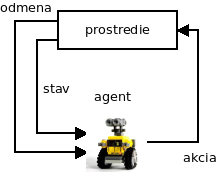
\includegraphics[scale=.4]{../diagrams/agent.png}
  \end{figure}

  \begin{figure}[!htb]
  \centering
  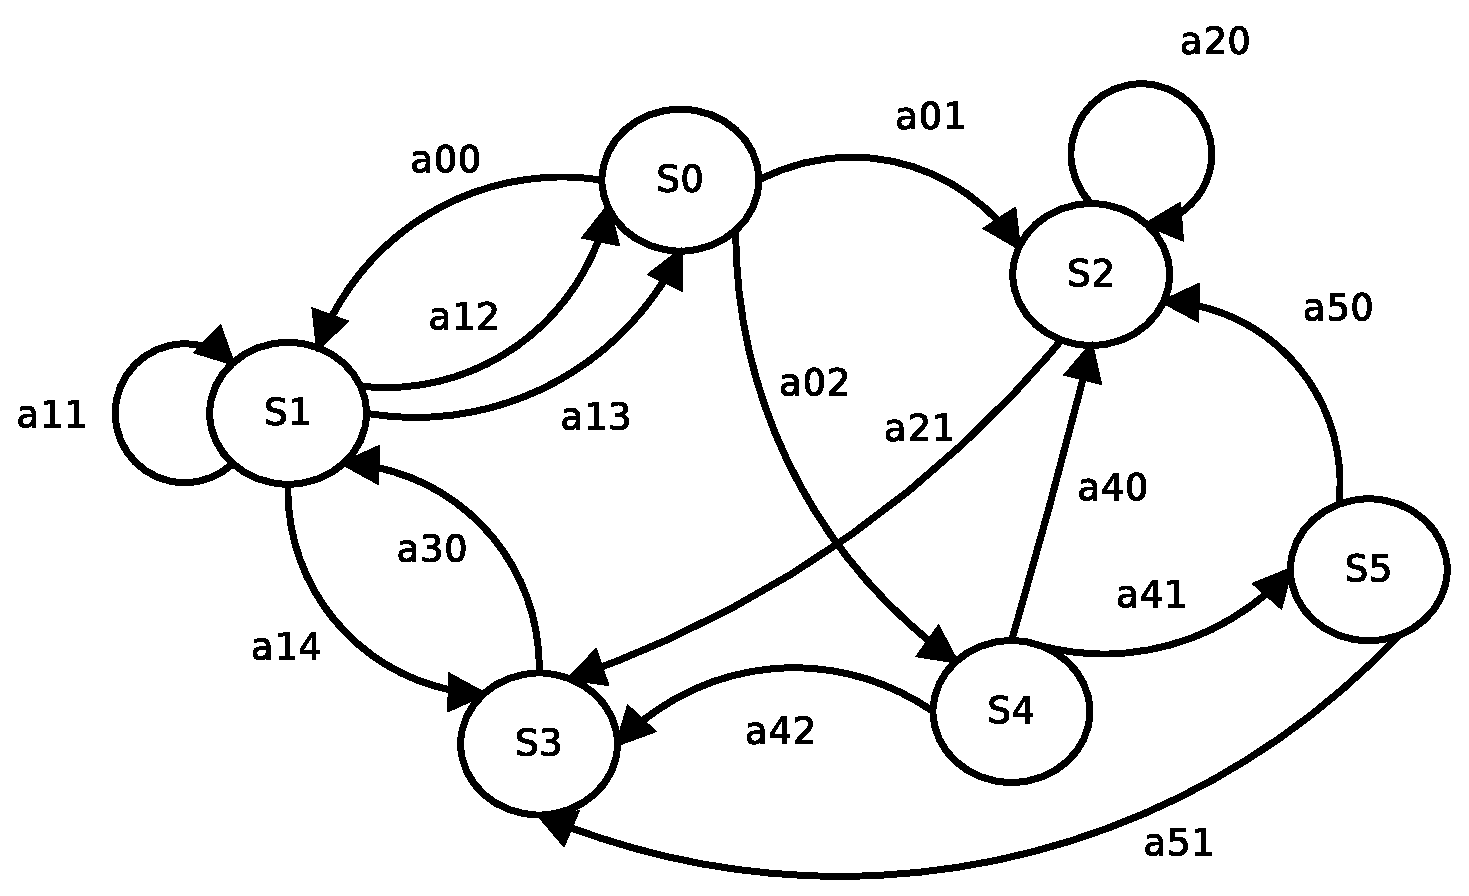
\includegraphics[scale=.2]{../diagrams/markovov_process.eps}
  \end{figure}

\end{minipage}

\end{frame}


%-------------------------------------------------------------------------------------
\begin{frame}{\bf Funkcia ohodnotení}

Daná je funkcia ohodnotení \\
{\footnotesize Watkins 1989, konvergencia k optimálnej stratégií : Melo, Even-Dar, Kearns : $\left( V = \sum\limits_{n=0}^{\infty} \gamma^n T(n) \right)$}

\begin{equation}
Q(s(n),a(n)) = R(s(n),a(n)) + \gamma \max_{a(n-1) \in \mathbb{A}} Q(s(n-1), a(n-1)) \nonumber
\label{eq:q_learning}
\end{equation}
kde \\

\begin{itemize}
 \item $R(s(n),a(n))$ je odmeňovacia funkcia \\
 \item $Q(s(n-1),a(n-1))$ je funkcia ohodnotení v stave $s(n-1)$ pre akciu $a(n-1)$, \\
 \item $\gamma$ je konštanta zabúdania a platí $\gamma \in (0, 1)$.
\end{itemize}

\begin{figure}[!htb]
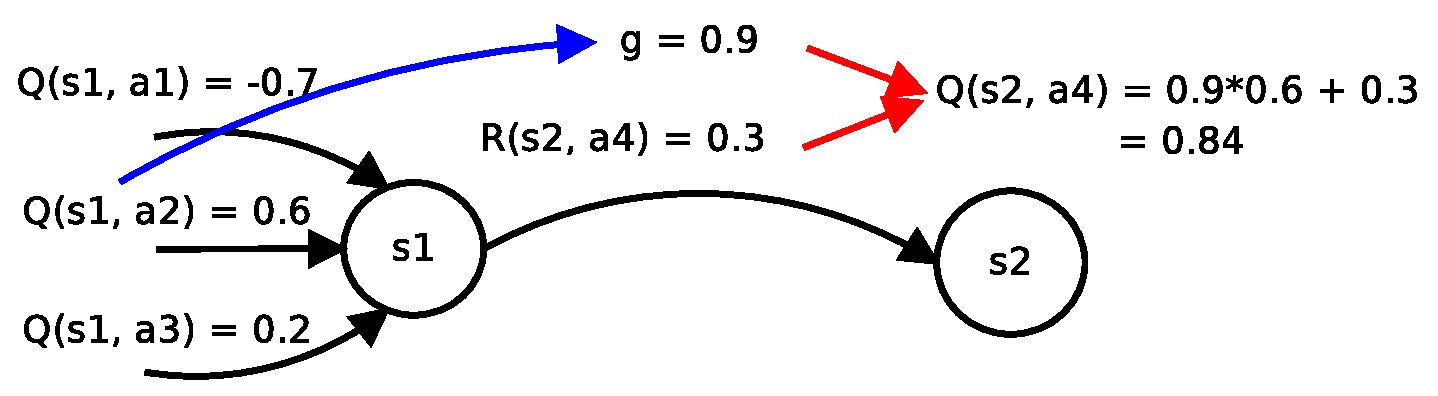
\includegraphics[scale=.4]{../diagrams/q_learning_detail.eps}
\end{figure}

\end{frame}

%-------------------------------------------------------------------------------------
\begin{frame}{\bf Konštanta zabúdania }

  \begin{figure}[!htb]
  \centering
  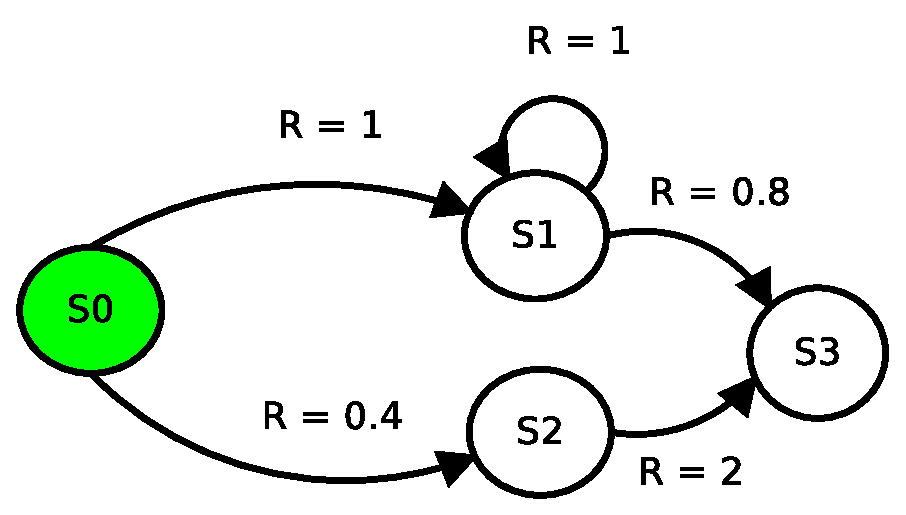
\includegraphics[scale=.5]{../diagrams/rf_cycle_states.eps}
  \end{figure}

  Ohodnotenie ciest :
  \begin{itemize}
    \item $S(S0, S2, S3) = 2 + 0.9*0.4 = 2.36$
    \item $S(S0, S1, S3) = 1 + 0.9*1 = 1.9$
    \item $S(S0, S1, S1, S1) = 1 + 0.9*(1 + 0.9*1) = 2.71 $
    \item $S(S0, S1, S1, S1, S1) = 1 + 0.9*(1 + 0.9*(1 + 0.9*1)) = 3.439$
    \item $S(S0, S1, S1, S1, S1, S1, ...) = 10$ <-----
    \item $S(S0, S1, S1, S1, S1, S1, ..., S3) = 10.8$ <-----
  \end{itemize}

\end{frame}




%-------------------------------------------------------------------------------------
\begin{frame}{\bf Cieľ práce}

\begin{block}{Problémy interpretácie $Q(s(n), a(n))$}
  \vspace{-2mm}
  {\footnotesize (Philip Sabes 1996, Melo 2007, Alborz Geramifard 2013)}
  \vspace{-1mm}
  \begin{itemize}
    \vspace{-1mm}
    \item pre veľké počty stavov, mnohorozmerné stavové priestory alebo veľký počet akcíí narastajú pamäťové nároky

          \begin{itemize}
          \item robot s 20 senzormi kde každý má 256 hodnôt sa môže nachádzať v $1.46*10^{48}$ stavoch
          \item odhadovaný počet atómov v pozorovateľnom vesmíre je $10^{80}$
          \end{itemize}

    \vspace{-1mm}
    \item o nevyplnených $Q(s(n), a(n))$ nevieme povedať nič

    \vspace{-1mm}
    \item pre rozsiahle stavové priestory ťažko vypočítateľné

    \vspace{-1mm}
    \item ako aproximovať $Q(s(n), a(n))$?

  \end{itemize}

\end{block}

\vspace{-3mm}

\begin{exampleblock}{Používané prístupy}
  \vspace{-3mm}
  \begin{itemize}

  \vspace{-1mm}
  \item tabuľka

  \vspace{-1mm}
  \item bázické funkcie {\footnotesize (Sabes, Menache,  Keller)}

  \vspace{-1mm}
  \item sparse distributed memory {\footnotesize (Kenerva, Hawkins)}
  \end{itemize}
\end{exampleblock}


\vspace{-3mm}

\begin{alertblock}{Cieľ : aproximovať funkciu $Q(s(n), a(n))$}
  \vspace{-3mm}
  \begin{itemize}

  \vspace{-1mm}
  \item rýchle učenie

  \vspace{-1mm}
  \item kvalita riešenia
  \end{itemize}
\end{alertblock}

\end{frame}


%-------------------------------------------------------------------------------------
\begin{frame}{\bf Aproximácia doprednou perceptronovou neurónovou sieťou}

Utopická predstava : \\
{\footnotesize (Sebastian Thrun 1993, Leemon Baird N/A, Silvia Ferrari 2005, Ma Yumei 2012) }

\begin{figure}[!htb]
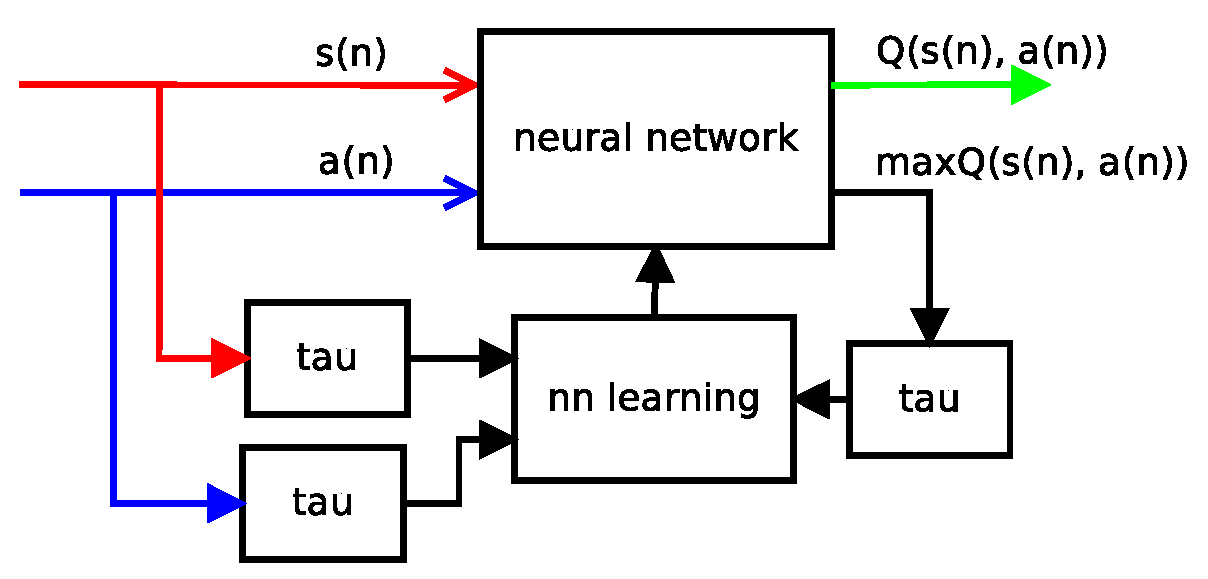
\includegraphics[scale=.5]{../diagrams/q_learning_nn.eps}
\end{figure}

Prečo nedáva správne výsledky?
\end{frame}

%-------------------------------------------------------------------------------------
\begin{frame}{\bf Hypotéza}

Na základe experimetov - Snowball problém

\begin{figure}[!htb]
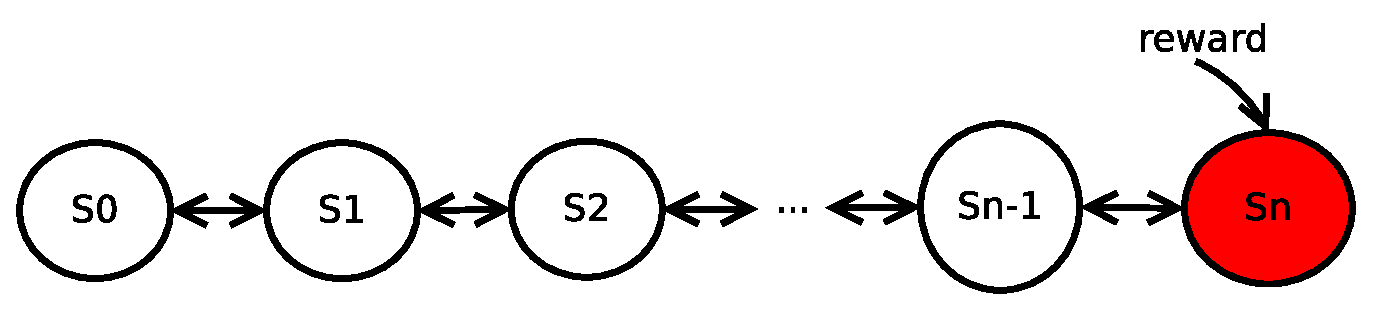
\includegraphics[scale=.5]{../diagrams/q_chain_problem.eps}
\end{figure}

Pre korektné vyplnenie hodnôt v $s_{n-1}$ sa vyžaduje korektá hodnota v $s_{n}$

\begin{align*}
    Q(s(1),a(1)) &= R(s(1),a(1)) + \gamma \max_{a(0) \in \mathbb{A}} Q(s(0), a(0)) \\
    Q(s(2),a(2)) &= R(s(2),a(2)) + \gamma \max_{a(1) \in \mathbb{A}} Q(s(1), a(1)) \\
    & \dots
\end{align*}

\end{frame}




%-------------------------------------------------------------------------------------
\begin{frame}{\bf Rozklad $Q(s(n), a(n))$ na bázické funkcie}
Vzhľadom na charakter učiaceho algoritmu
\begin{equation} \label{eu_eqn}
Q(s(n),a(n)) = R(s(n),a(n)) + \gamma \max_{a(n-1) \in \mathbb{A}} Q(s(n-1), a(n-1)) \nonumber
\end{equation}
\begin{minipage}{.5\textwidth}
  boli zvolené bázické funkcie % (parameter $n$ pre prehľadnosť vynechaný)
  \begin{align*}
  f_j^1(\boldmath{s, a}) &= e^{ -\sum\limits_{i=1}^{n_s}{\beta_{aji}(s_i - \alpha_{aji})^2} } \\
  f_j^2(\boldmath{s, a}) &= \frac{1}{1 + \sum\limits_{i=1}^{n_s}{\beta_{aji}(s_i - \alpha_{aji})^2}} \\
  \end{align*}
\end{minipage}%
\begin{minipage}{.5\textwidth}

  \begin{figure}[!htb]
  \centering
  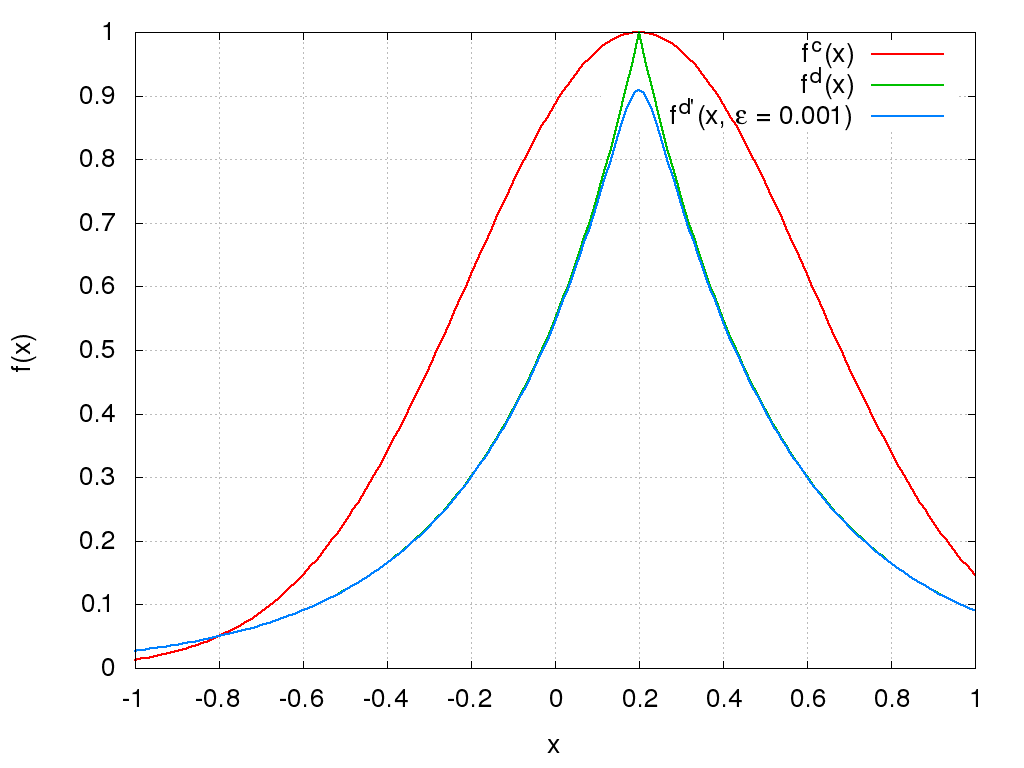
\includegraphics[scale=.2]{../pictures/gaussian_1D.png}
  \end{figure}

\end{minipage}

a ich lineárna kombinácia

\begin{align}
    Q^x(s(n), a(n))&= \sum\limits_{j=1}^{l}w_{j a(n)}f^x_{j}(s(n), a(n)) \nonumber
\end{align}

\end{frame}


%-------------------------------------------------------------------------------------
\begin{frame}{\bf Nová bázická funkcia}

Tabuľka pre vybrané hodnoty (adaptívna tabuľka - AT)- umožní zachytit skokovú zmenu \\
Gaussova krivka - dokáže pokryť nenulovými hodnotami celý definičný obor \\

\begin{align}
P_i(s(n), a(n)) &=
\left\{
	\begin{array}{ll}
		r_{ai}  & ak \ s(n) = \alpha^1_i \\
		0 & inak
	\end{array}
\right. \\
  H_j(s(n), a(n)) &= w_{aj} e^{ -\beta_{aj} \sum\limits_{i=1}^{n_s}{(s_i(n) - \alpha^2_{aji})^2 }} \\
  Q(s(n), a(n)) &= \sum\limits_{i=1}^{I} P_i(s(n),a(n)) + \sum\limits_{j=1}^{J} H_j(s(n), a(n))
  \label{eq:peak_hill}
\end{align}


\end{frame}


%-------------------------------------------------------------------------------------
\begin{frame}{\bf Nová bázická funkcia}

\begin{figure}[!htb]
\centering
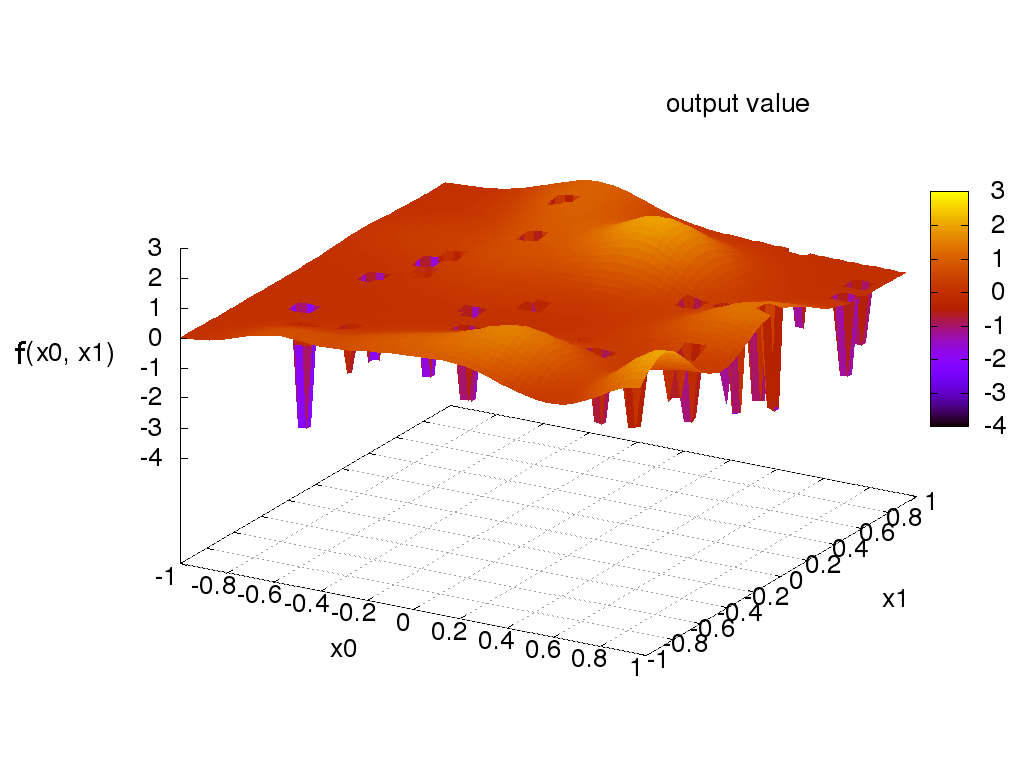
\includegraphics[scale=.4]{../pictures/peak_hill_function.png}
\end{figure}

\end{frame}







%-------------------------------------------------------------------------------------
\begin{frame}{\bf Bloková schéma syntézy testovaného riešenia}

\begin{figure}[!htb]
\centering
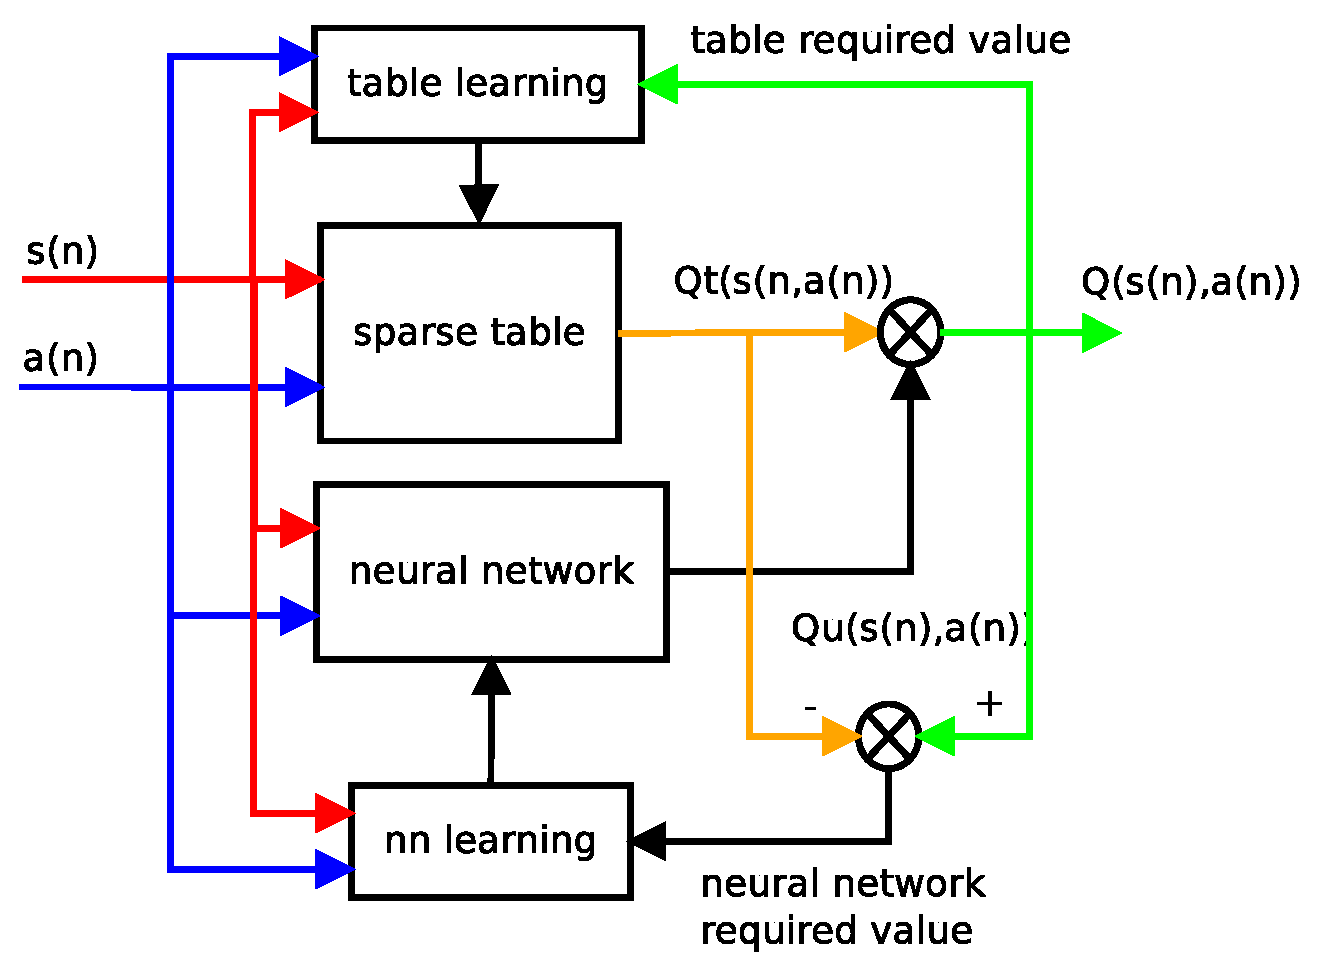
\includegraphics[scale=.4]{../diagrams/q_learning_hybrid.eps}
\end{figure}

\end{frame}

%-------------------------------------------------------------------------------------
\begin{frame}{\bf Schéma priebehu experimentov}

\begin{figure}[!htb]
\centering
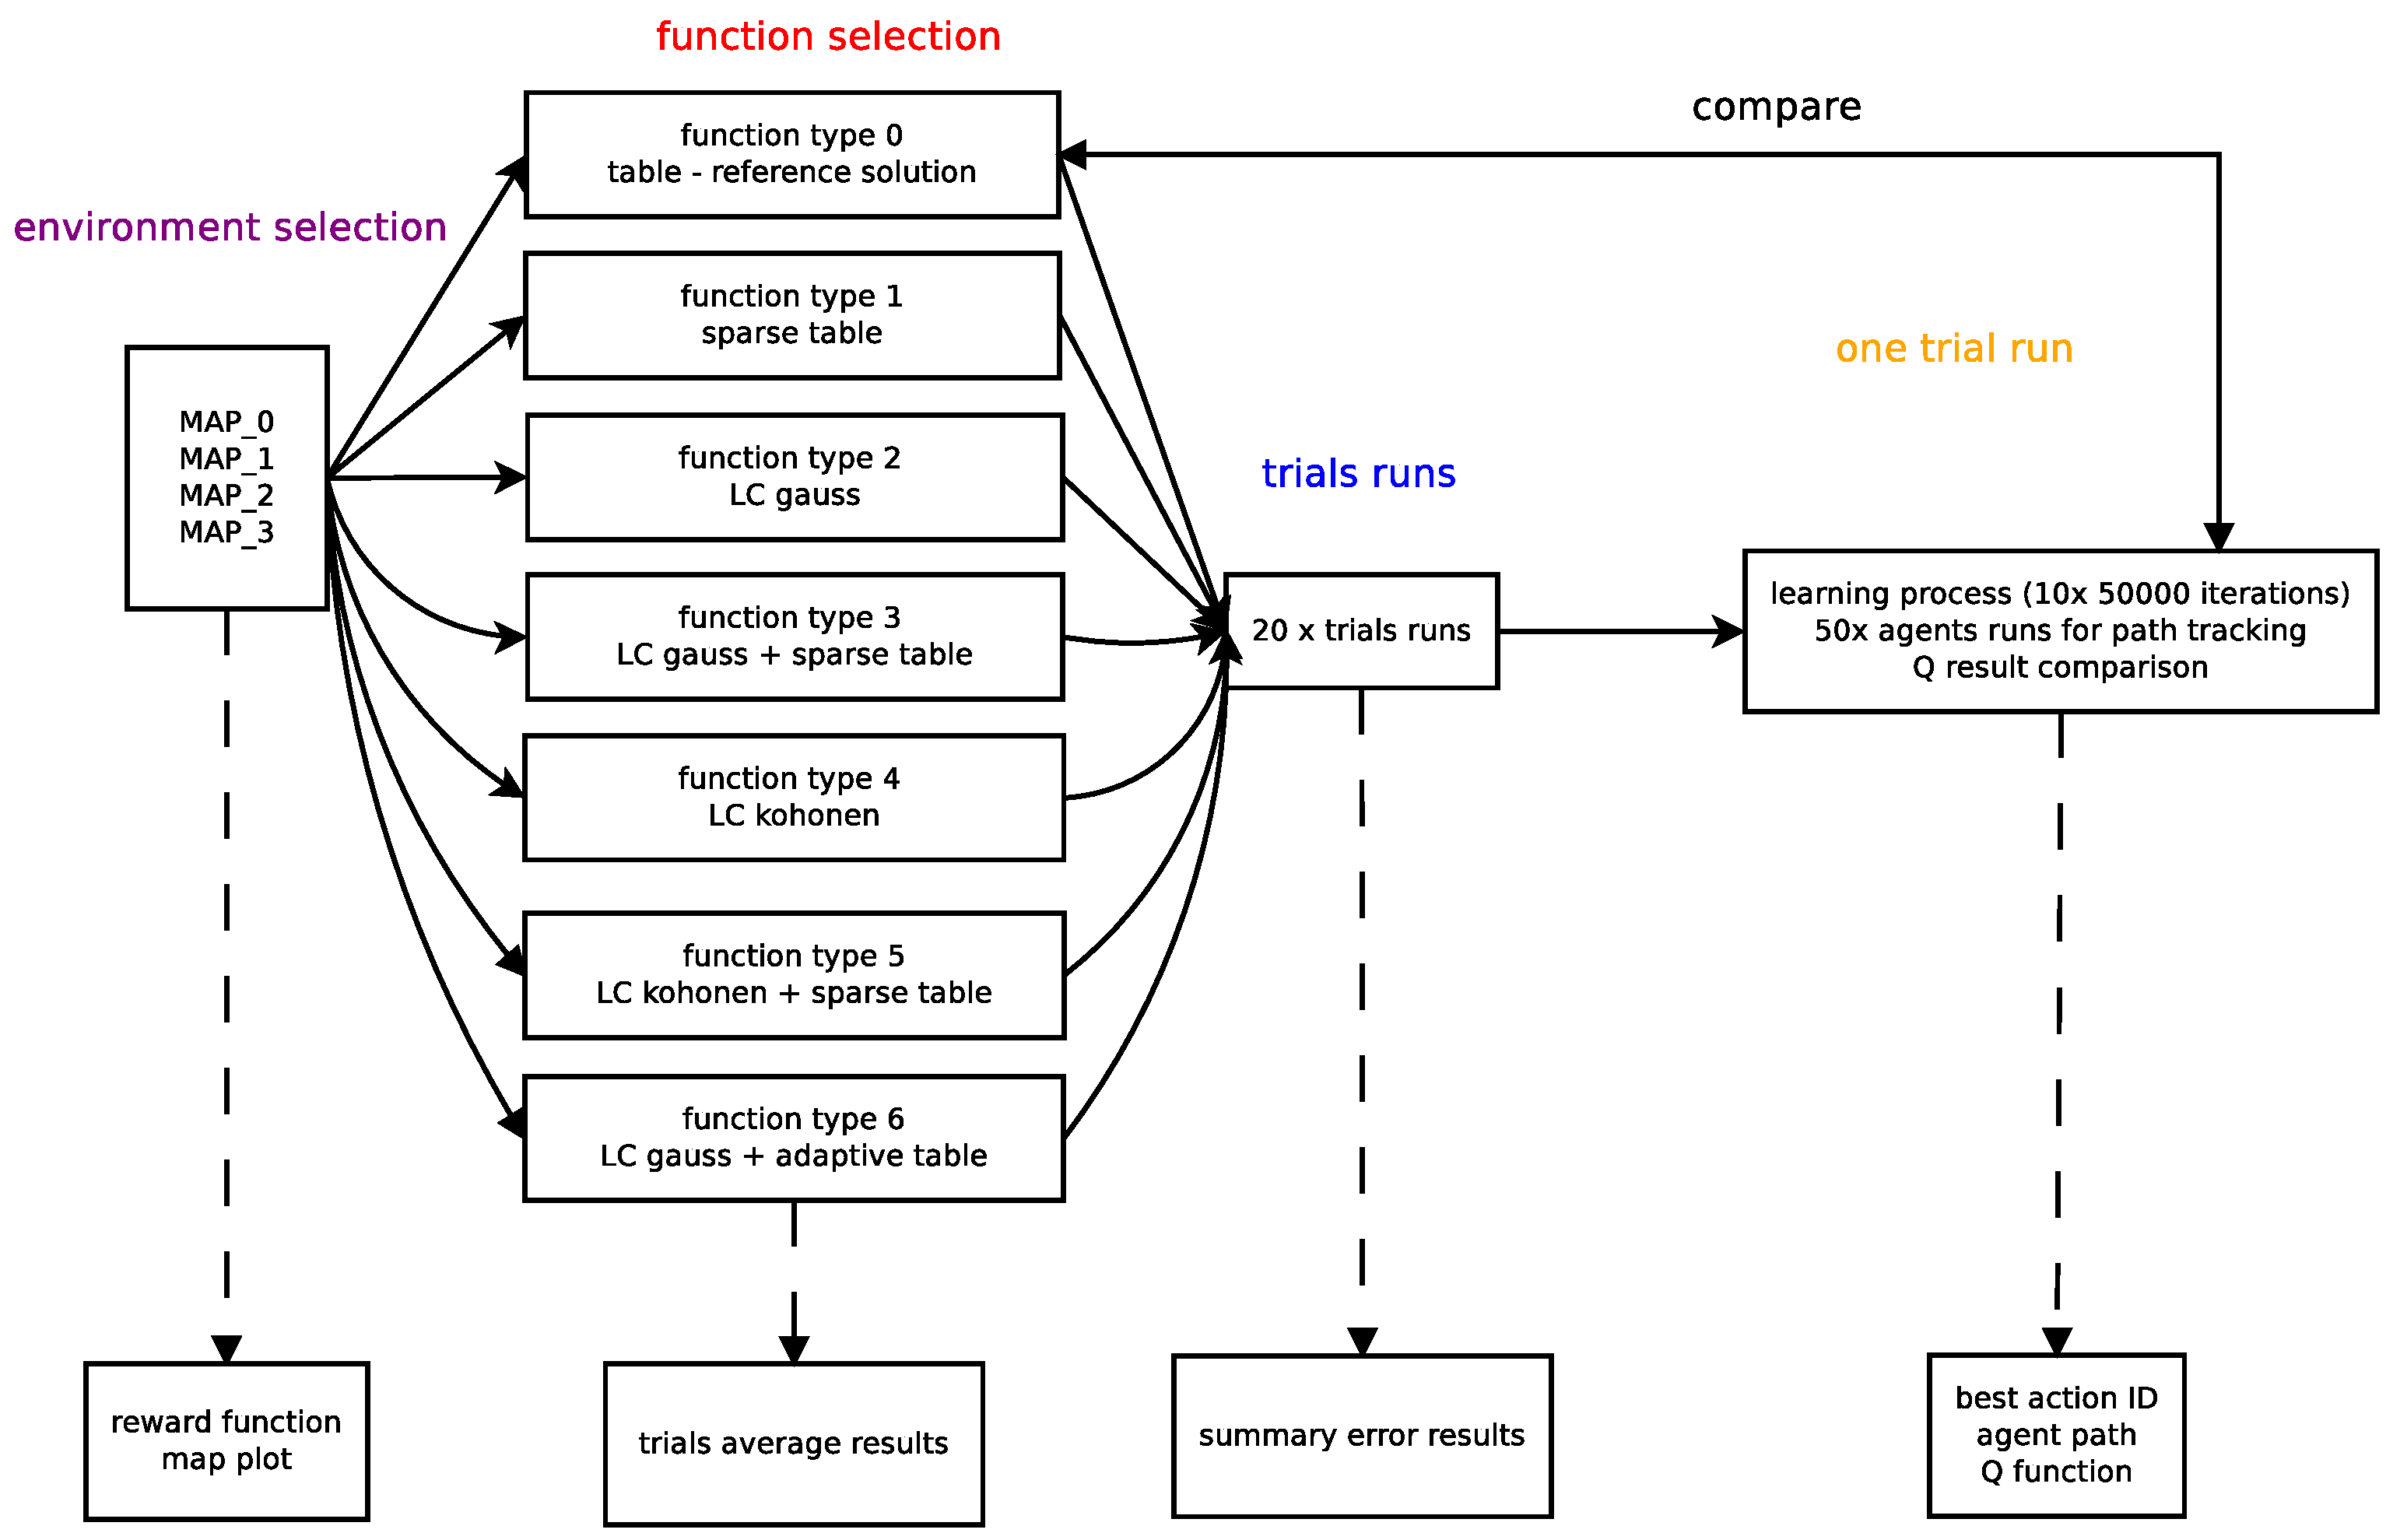
\includegraphics[scale=.22]{../diagrams/experiment_map_q_learning.eps}
\end{figure}

\end{frame}





%-------------------------------------------------------------------------------------
\begin{frame}{\bf Návrh experimentov - podmienky}

\begin{itemize}
\item 50000 iterácií učenia
\item rozmer $s$ je $n_s = 2$, rozmer $a$ je $n_a = 2$
\item predpis funkcie ohodnotení
\begin{align}
&Q(s(n),a(n)) = \nonumber \\
&\alpha Q(s(n-1),a(n-1)) \nonumber \\
&(1- \alpha)(R(s(n),a(n)) + \gamma \max_{a(n-1) \in \mathbb{A}} Q(s(n-1), a(n-1)) \nonumber
\end{align}

\item $R(s(n), a(n)) \in \langle -1, 1 \rangle$ náhodné prostredie (mapa) s 1 cieľovým stavom
\item $\gamma = 0.98$ a $\alpha = 0.7$
\item hustota referenčného riešenia = 1/32  (4096 stavov)
\item počet akcií v každom stave = 8
\item hustota riedkej tabuľky = 1/8  (1:16 pomer)
\item počet bázických funkcií $l = 64$
\item rozsah parametrov $\alpha_{ja}(n)$, $\beta_{ja}(n)$, $w_{ja}(n)$
\end{itemize}

\end{frame}


%-------------------------------------------------------------------------------------
\begin{frame}{\bf Návrh experimentov - podmienky}

$Q_{rt}(s(n),a(n))$ referenčná funkcia Q (funkcia r = 0), kde $t \in \langle 0, 19 \rangle $ je číslo trialu  \\
$Q_{jt}(s(n),a(n))$ testované funkcie Q a $j \in \langle 1, 5 \rangle $. \\

Celková chyba behu trialu $t$ je \\
\begin{equation}
e_{jt} = \sum\limits_{s, a}{(Q_{rt}(s,a) - Q_{jt}(s,a))^2}  \nonumber
\end{equation}

priemerná, minimálna, maximálna chyba a smerodajná odchylka \\
\begin{align}
\bar{a_j} &= \frac{1}{20}\sum\limits_{t}{e_{jt}}  \nonumber \\
{e^{min}_j} &= \min_{t}{e_{jt}}  \nonumber \\
{e^{max}_j} &= \max_{t}{e_{jt}}  \nonumber \\
{\sigma_j}^2 &= \frac{1}{20}\sum\limits_{t}{(\bar{a_j} - e_{jt})^2}  \nonumber
\end{align}

\end{frame}


%-------------------------------------------------------------------------------------
\begin{frame}{\bf Funkcia R(s, a), prostredie 2 - Výsledky experimentov}
Pre každý stav je zvolená rovnaka množina akcií. \\
Ďalej platí $s = (s[0], s[1])$.

\begin{figure}[!htb]
\centering
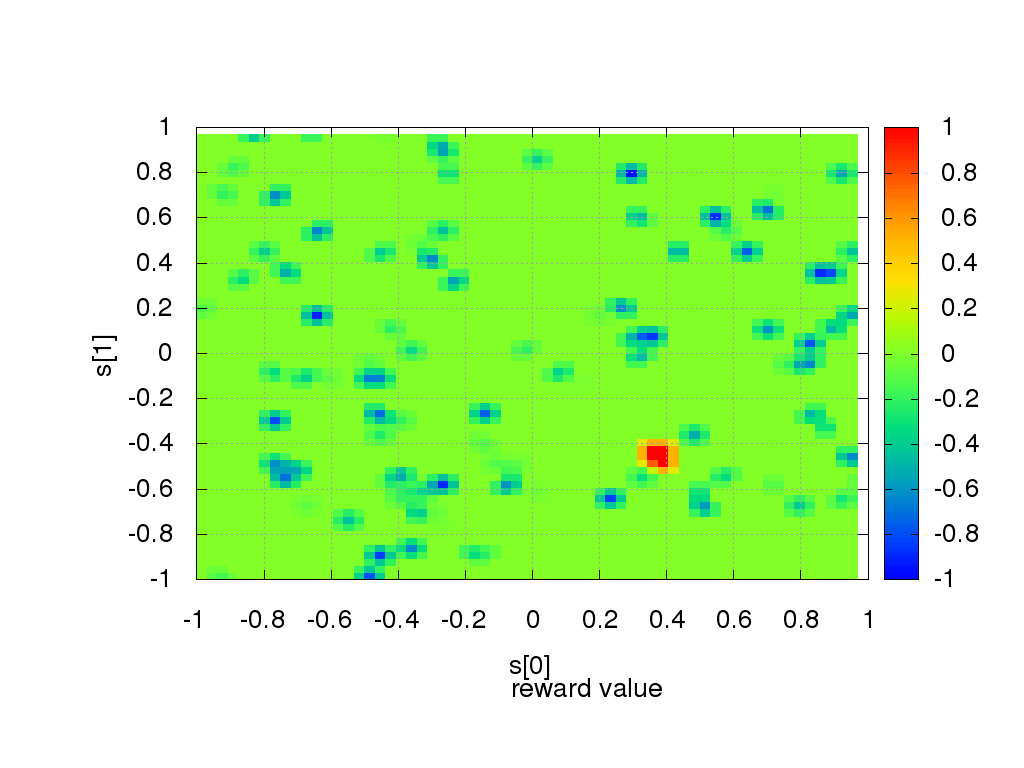
\includegraphics[scale=.35]{../../results_q_learning/map_2/reward_value_surface.png}
\end{figure}

\end{frame}



%-------------------------------------------------------------------------------------
\begin{frame}{\bf Mapa najlepších akcií - Výsledky experimentov}

Funkcia voľby najlepšej z 8 akcií v stave  $s = (s[0], s[1])$.

\begin{minipage}{.5\textwidth}

\begin{figure}[!htb]
\centering
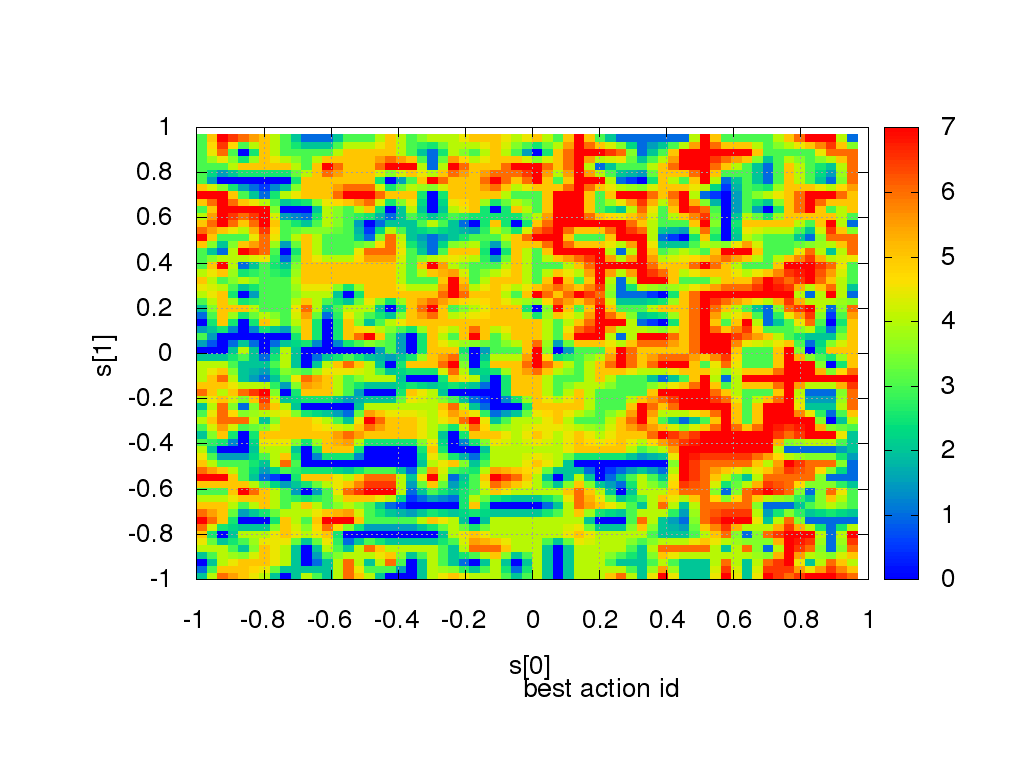
\includegraphics[scale=.21]{../../results_q_learning/map_2/function_type_0/iterations_10/action_best_value_log_surface.png}
\caption{reference solution}
\end{figure}

\end{minipage}%
\begin{minipage}{.5\textwidth}

\begin{figure}[!htb]
\centering
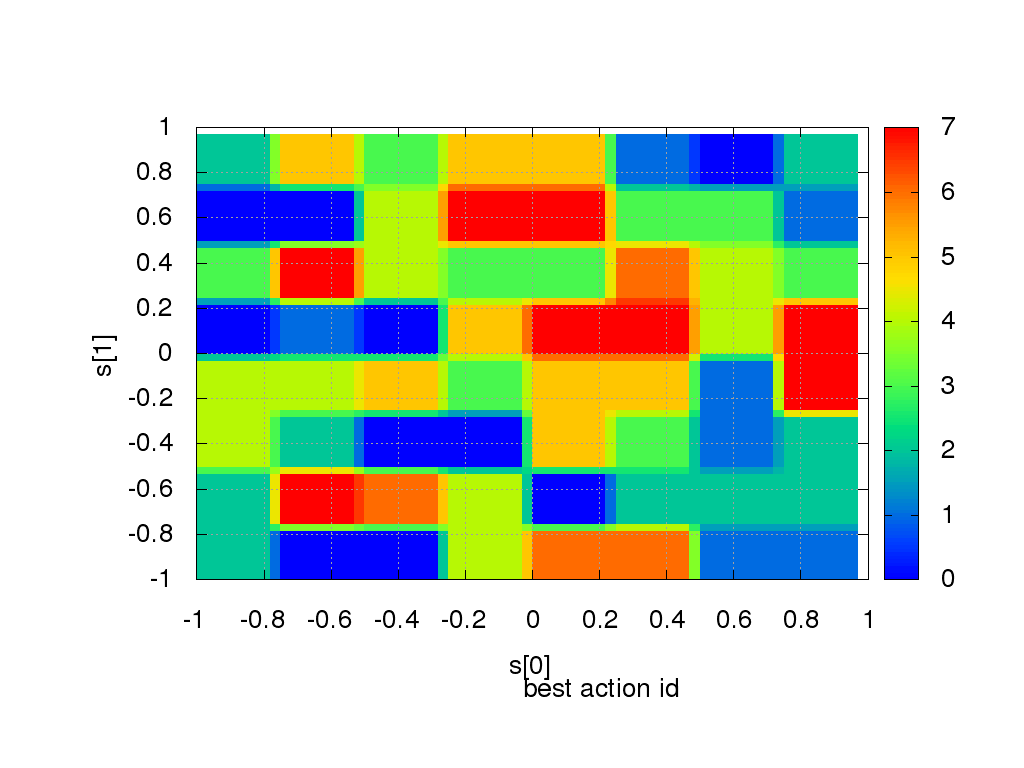
\includegraphics[scale=.21]{../../results_q_learning/map_2/function_type_1/iterations_10/action_best_value_log_surface.png}
\caption{sparse table}
\end{figure}


\end{minipage}
\end{frame}


%-------------------------------------------------------------------------------------
\begin{frame}{\bf Mapa najlepších akcií - Výsledky experimentov}

Funkcia voľby najlepšej z 8 akcií v stave  $s = (s[0], s[1])$.

\begin{minipage}{.5\textwidth}

\begin{figure}
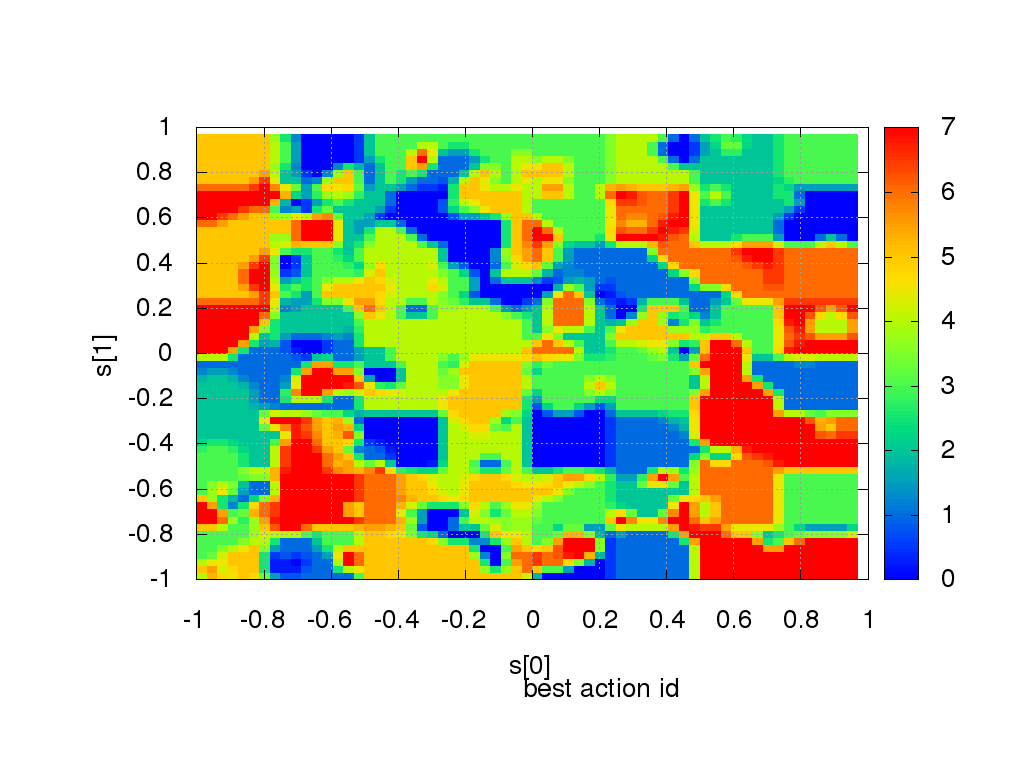
\includegraphics[scale=.21]{../../results_q_learning/map_2/function_type_3/iterations_10/action_best_value_log_surface.png}
\caption{sparse table + linear combination Gauss}
\end{figure}


\end{minipage}%
\begin{minipage}{.5\textwidth}

\begin{figure}
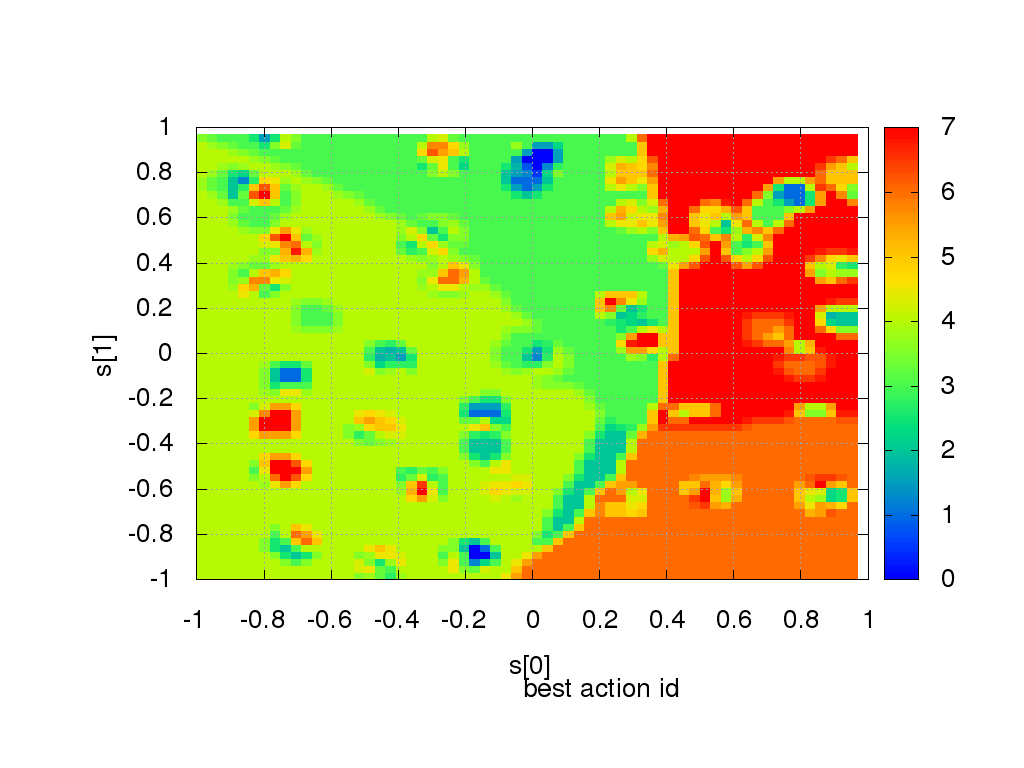
\includegraphics[scale=.21]{../../results_q_learning/map_2/function_type_6/iterations_10/action_best_value_log_surface.png}
\caption{adaptive table + linear combination Gauss}
\end{figure}


\end{minipage}
\end{frame}









\begin{frame}{\bf Dráhy agentov pri voľbe najlepšej akcie}

\begin{minipage}{.5\textwidth}

  \begin{figure}[!htb]
  \centering
  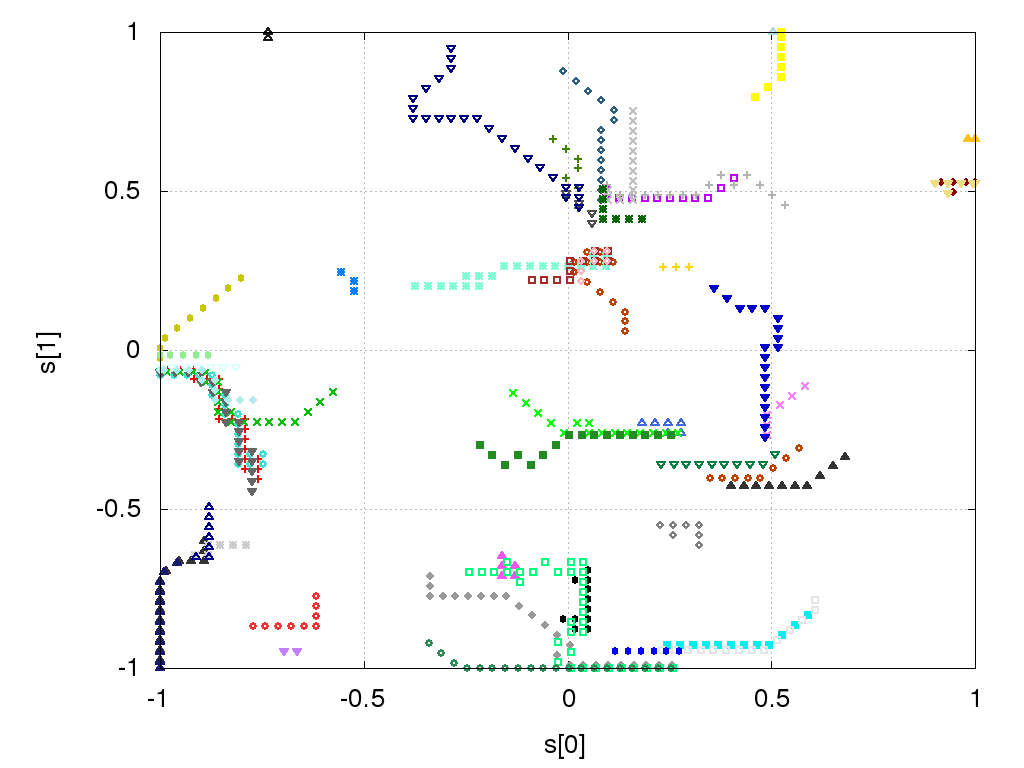
\includegraphics[scale=.2]{../../results_q_learning/map_2/function_type_3/iterations_10/agents_path_surface.png}
  \caption{sparse table + linear combination Gauss}
  \end{figure}


\end{minipage}%
\begin{minipage}{.5\textwidth}

  \begin{figure}[!htb]
  \centering
  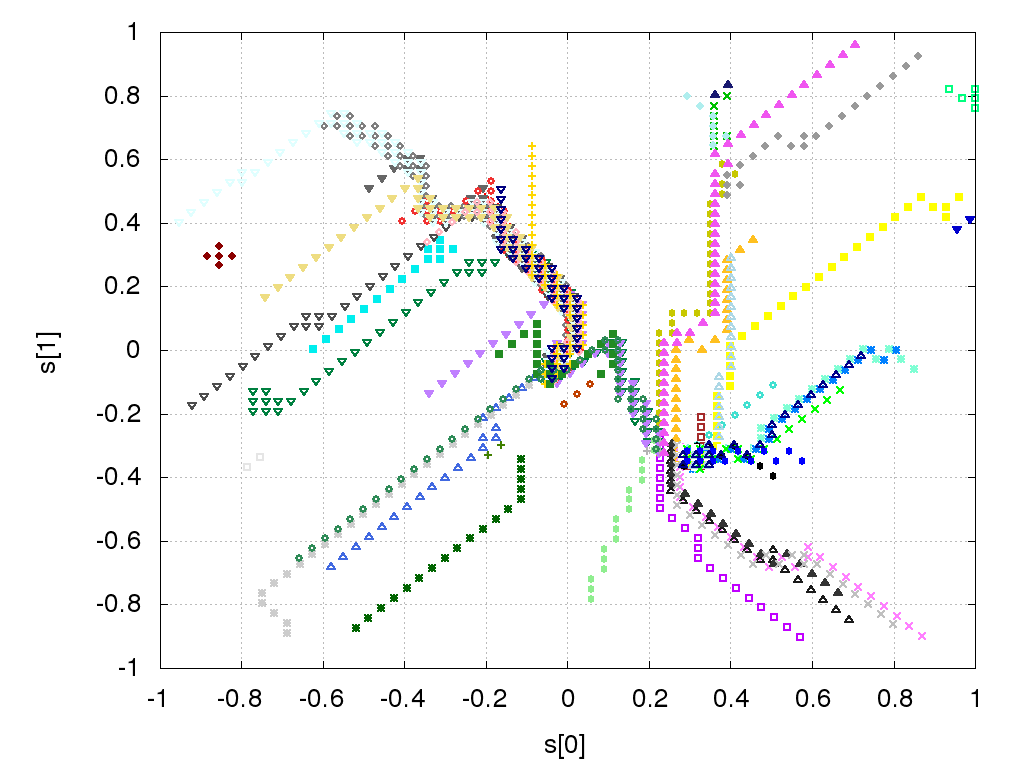
\includegraphics[scale=.2]{../../results_q_learning/map_2/function_type_6/iterations_10/agents_path_surface.png}
  \caption{adaptive table + linear combination Gauss}
  \end{figure}

\end{minipage}

\end{frame}




%-------------------------------------------------------------------------------------
\begin{frame}{\bf Chybové funkcie - Výsledky experimentov}

\begin{equation}
e_{jt}(s) = (Q_{rt}(s,a) - Q_{jt}(s,a))^2  \nonumber
\end{equation}

\begin{minipage}{.5\textwidth}

\begin{figure}[!htb]
\centering
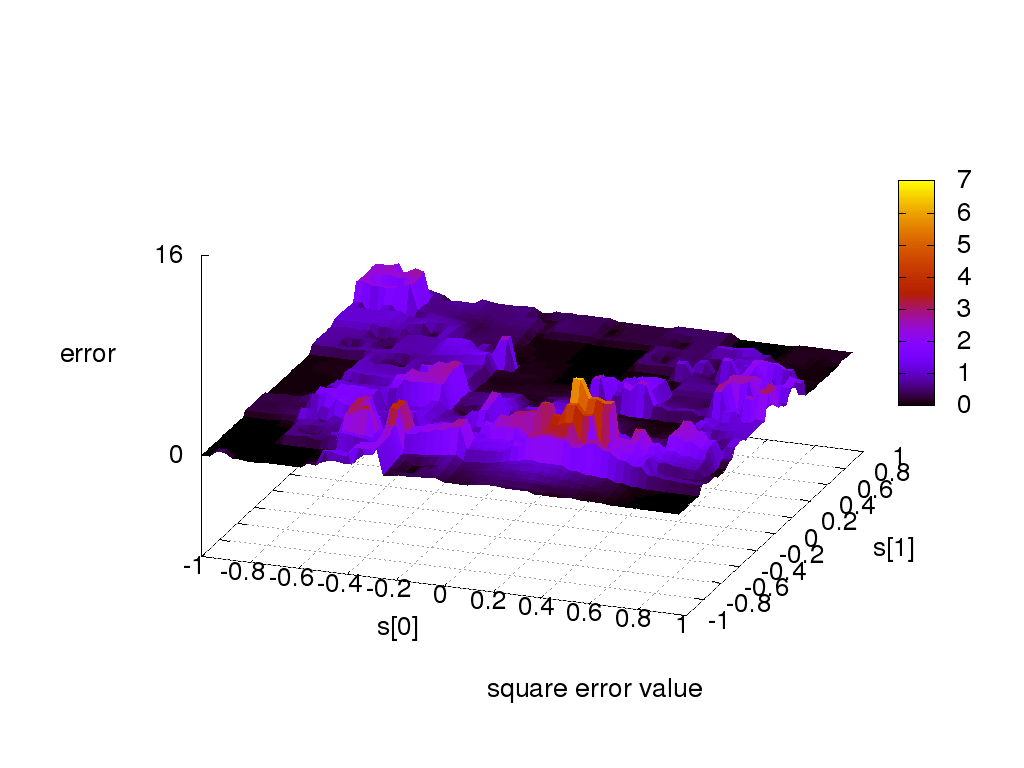
\includegraphics[scale=.2]{../../results_q_learning/map_2/function_type_3/q_learning_error.png}
\caption{sparse table + linear combination Gauss}
\end{figure}

\end{minipage}%
\begin{minipage}{.5\textwidth}

\begin{figure}[!htb]
\centering
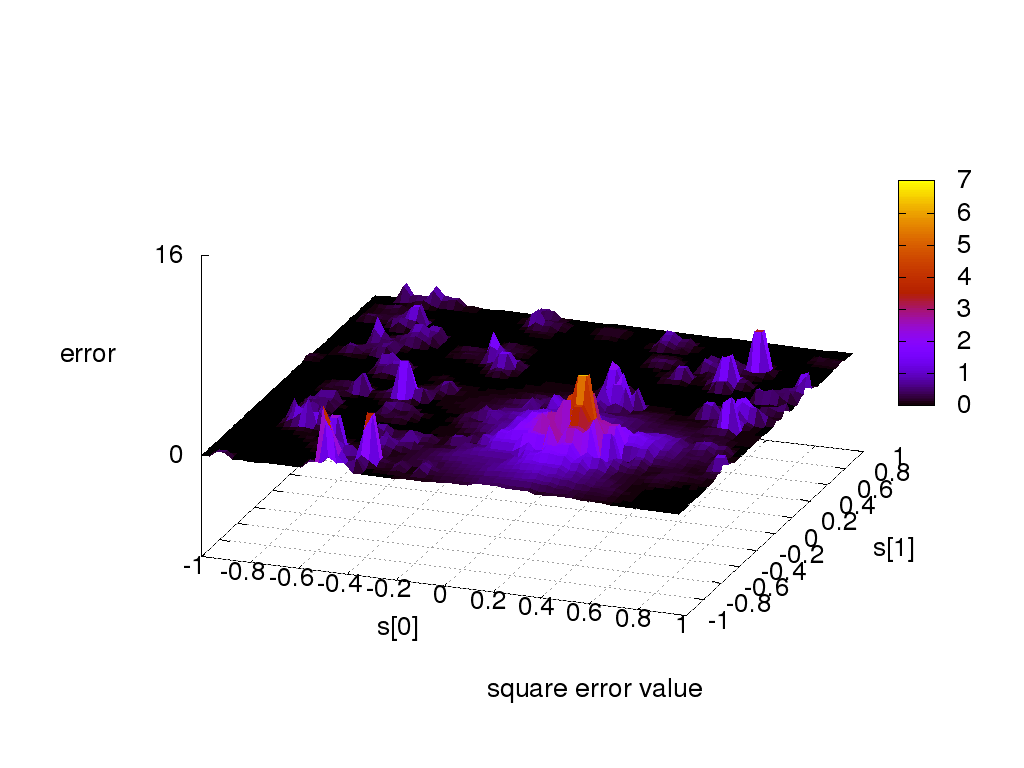
\includegraphics[scale=.2]{../../results_q_learning/map_2/function_type_6/q_learning_error.png}
\caption{adaptive table + linear combination Gauss}
\end{figure}


\end{minipage}
\end{frame}


%-------------------------------------------------------------------------------------
\begin{frame}{\bf max Q(s, a) - Výsledky experimentov}

\begin{minipage}{.5\textwidth}

\begin{figure}[!htb]
\centering
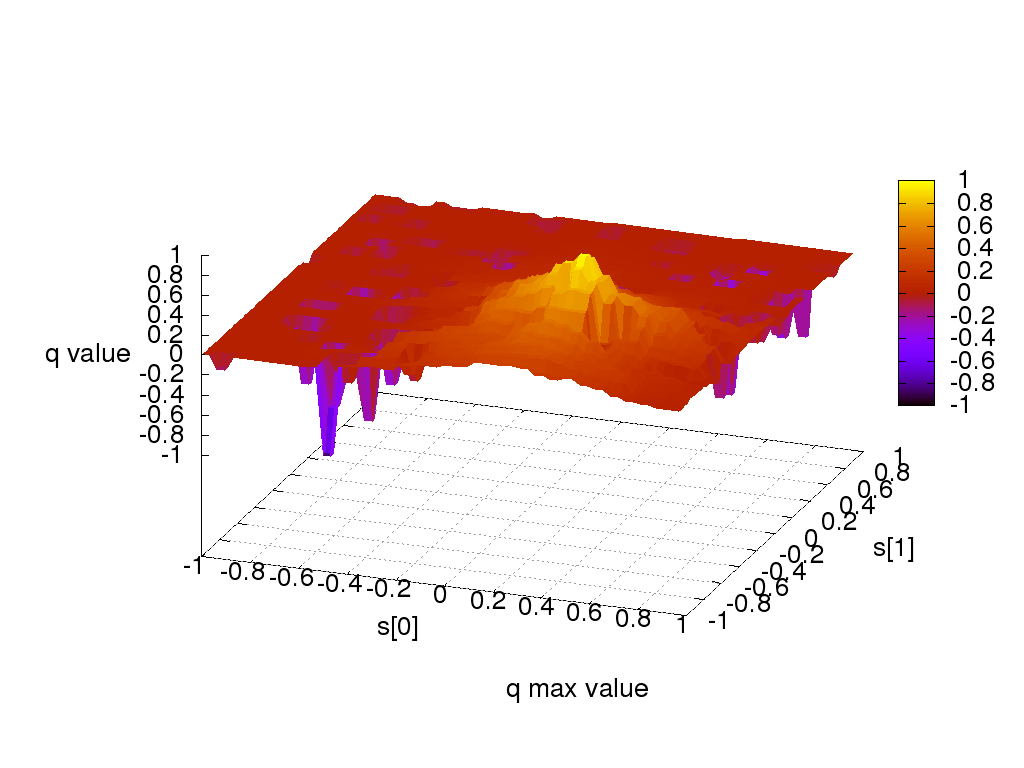
\includegraphics[scale=.2]{../../results_q_learning/map_2/function_type_0/iterations_10/q_learning_result.png}
\caption{reference table}
\end{figure}

\end{minipage}%
\begin{minipage}{.5\textwidth}

\begin{figure}[!htb]
\centering
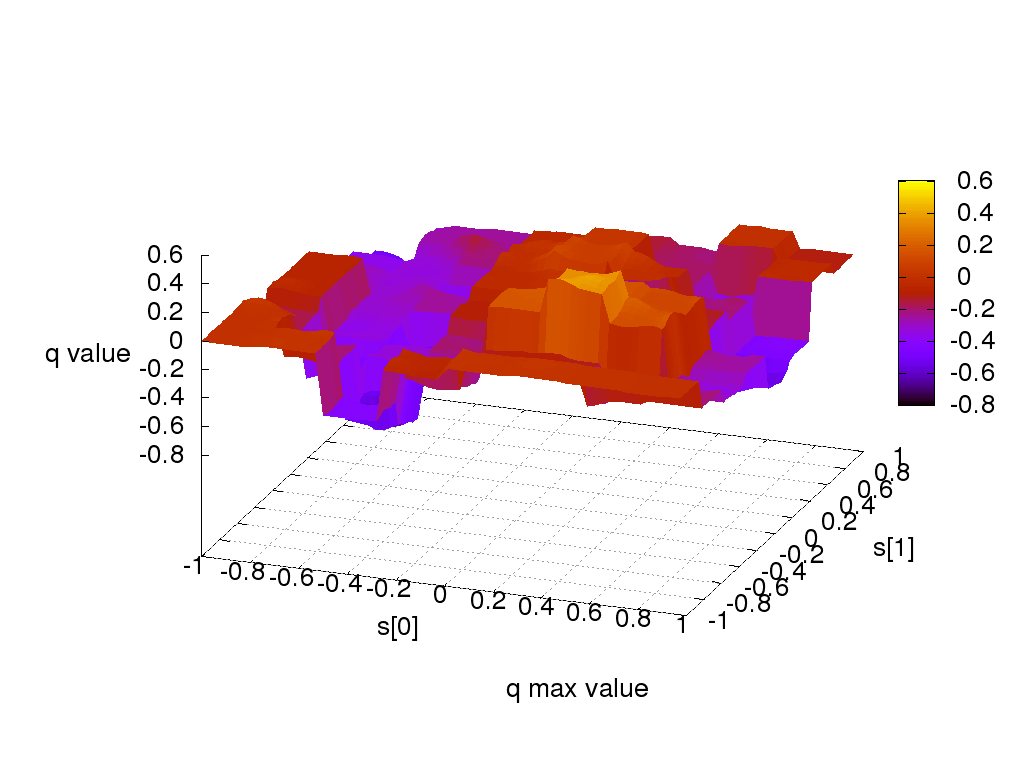
\includegraphics[scale=.2]{../../results_q_learning/map_2/function_type_3/iterations_10/q_learning_result.png}
\caption{sparse table + linear combination Gauss}
\end{figure}


\end{minipage}
\end{frame}





%-------------------------------------------------------------------------------------
\begin{frame}{\bf max Q(s, a) - Výsledky experimentov}

\begin{minipage}{.5\textwidth}

\begin{figure}[!htb]
\centering
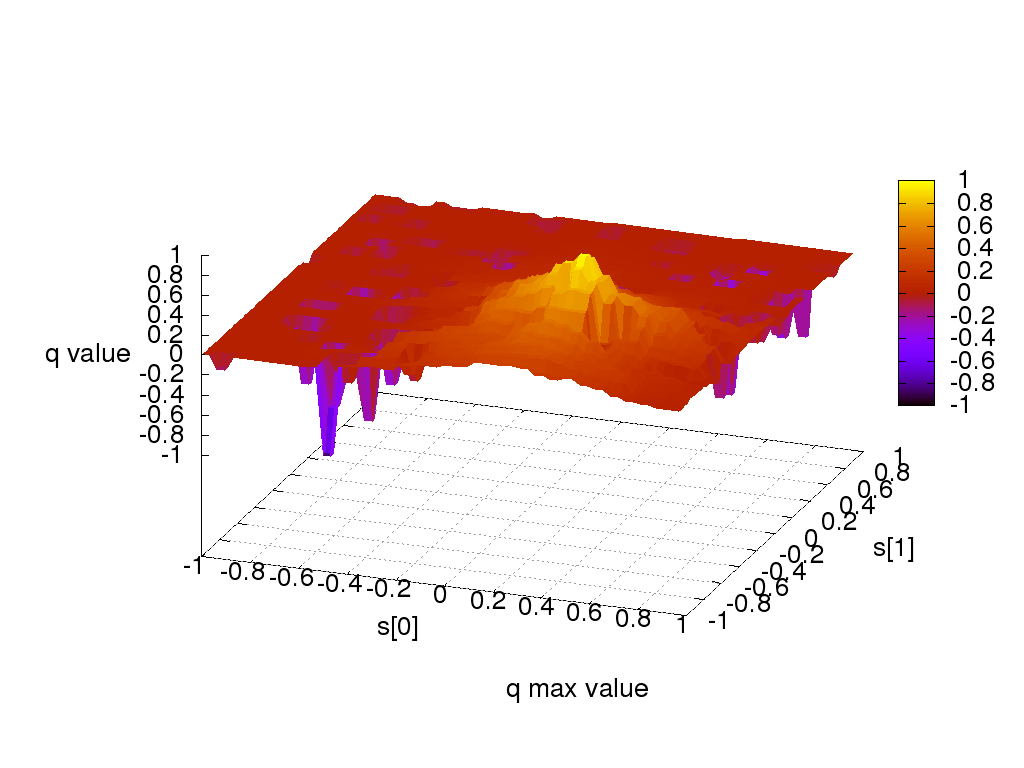
\includegraphics[scale=.2]{../../results_q_learning/map_2/function_type_0/iterations_10/q_learning_result.png}
\caption{reference table}
\end{figure}

\end{minipage}%
\begin{minipage}{.5\textwidth}

\begin{figure}[!htb]
\centering
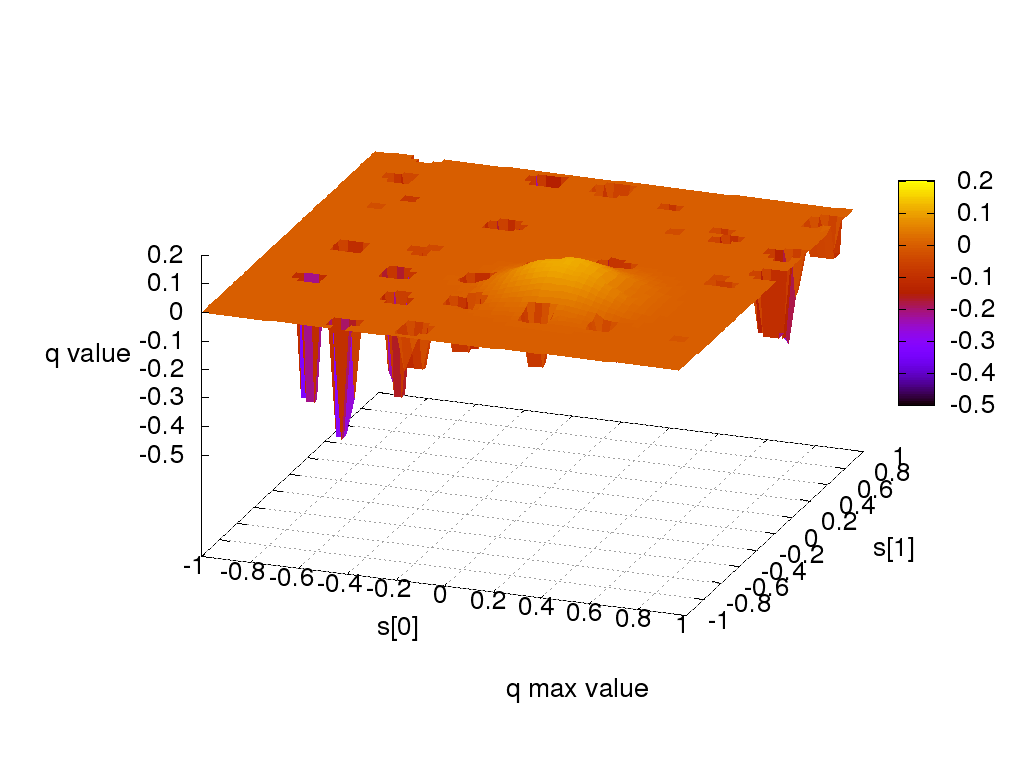
\includegraphics[scale=.2]{../../results_q_learning/map_2/function_type_6/iterations_10/q_learning_result.png}
\caption{adaptive table + linear combination Gauss}
\end{figure}


\end{minipage}
\end{frame}



%-------------------------------------------------------------------------------------
\begin{frame}{\bf Priebeh trialov - Výsledky experimentov}

\begin{figure}[!htb]
\centering
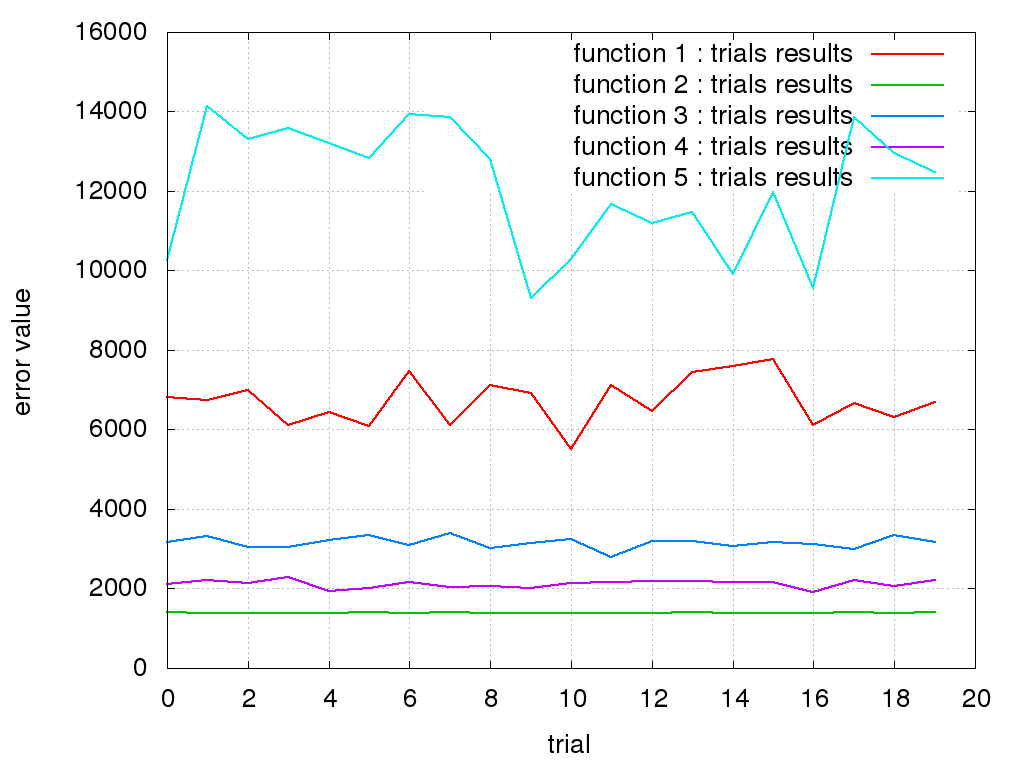
\includegraphics[scale=.36]{../../results_q_learning/map_2/trials_average_results_progress.png}
\end{figure}

\end{frame}



%-------------------------------------------------------------------------------------
\begin{frame}{\bf Prostredie 0 - Výsledky experimentov}

\begin{figure}[!htb]
\centering
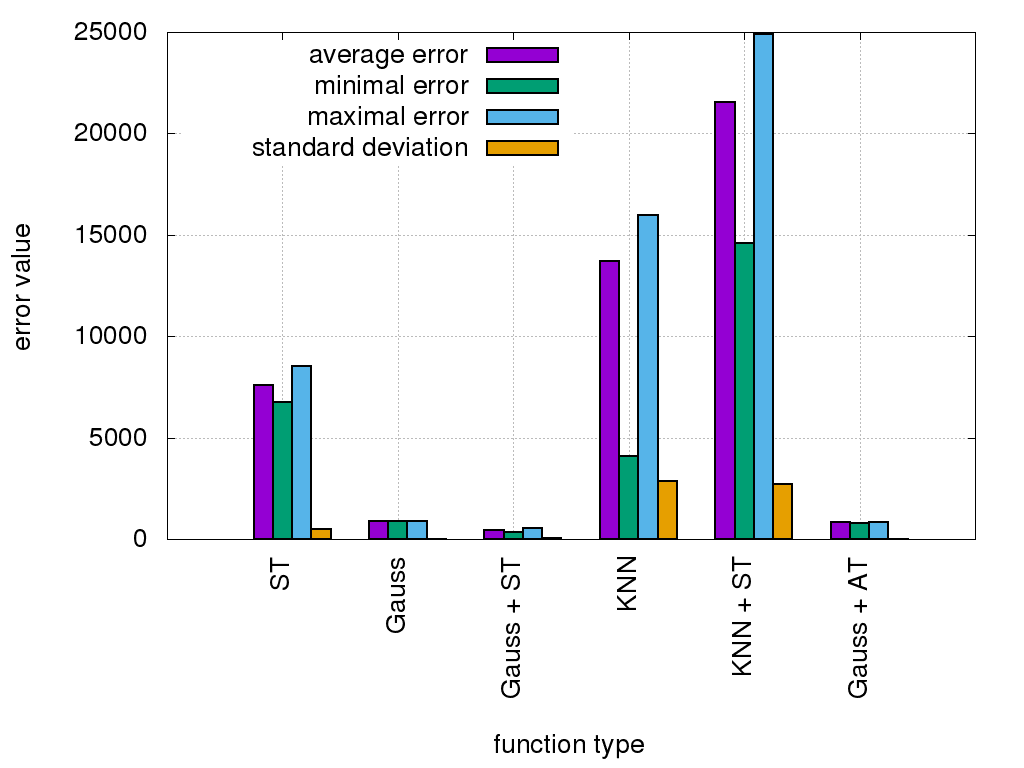
\includegraphics[scale=.36]{../../results_q_learning/map_0/trials_average_results.png}
\end{figure}

\end{frame}


%-------------------------------------------------------------------------------------
\begin{frame}{\bf Prostredie 1 - Výsledky experimentov}

\begin{figure}[!htb]
\centering
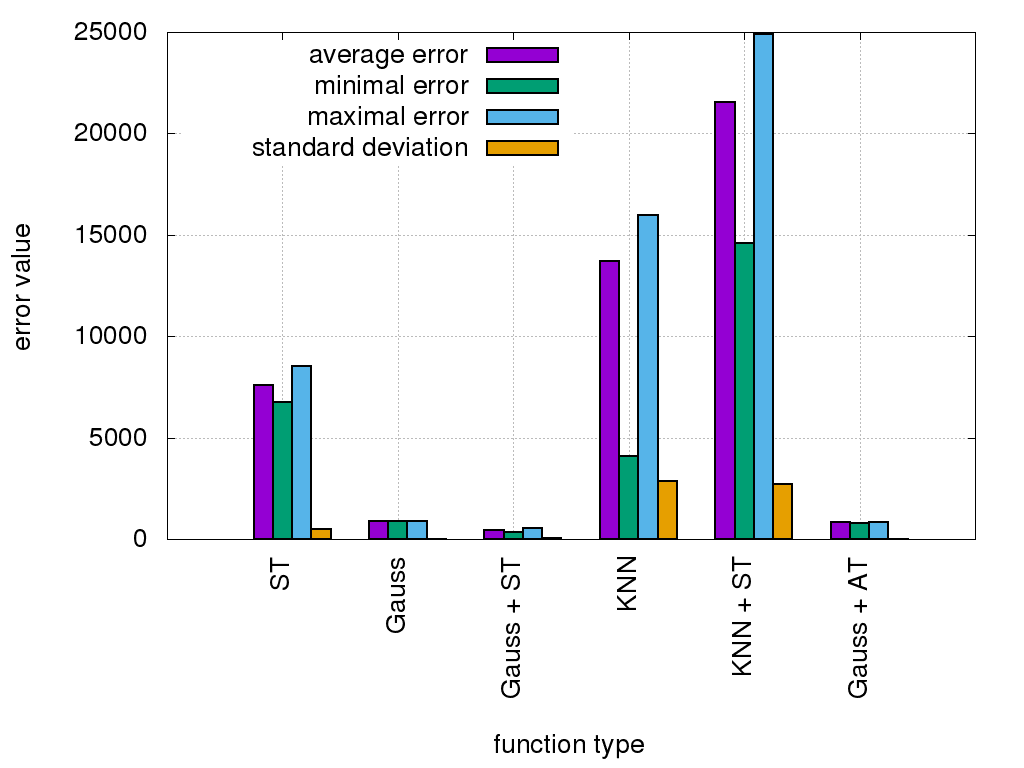
\includegraphics[scale=.36]{../../results_q_learning/map_0/trials_average_results.png}
\end{figure}

\end{frame}

%-------------------------------------------------------------------------------------
\begin{frame}{\bf Prostredie 2 - Výsledky experimentov}

\begin{figure}[!htb]
\centering
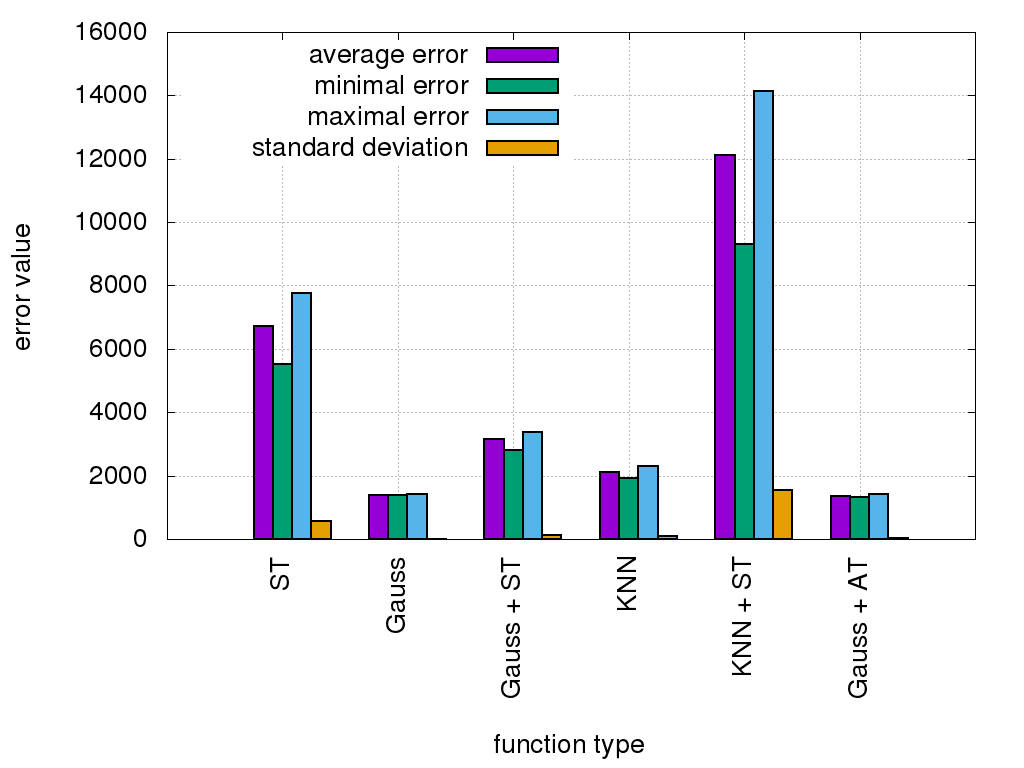
\includegraphics[scale=.36]{../../results_q_learning/map_2/trials_average_results.png}
\end{figure}

\end{frame}

%-------------------------------------------------------------------------------------
\begin{frame}{\bf Prostredie 3 - Výsledky experimentov}

\begin{figure}[!htb]
\centering
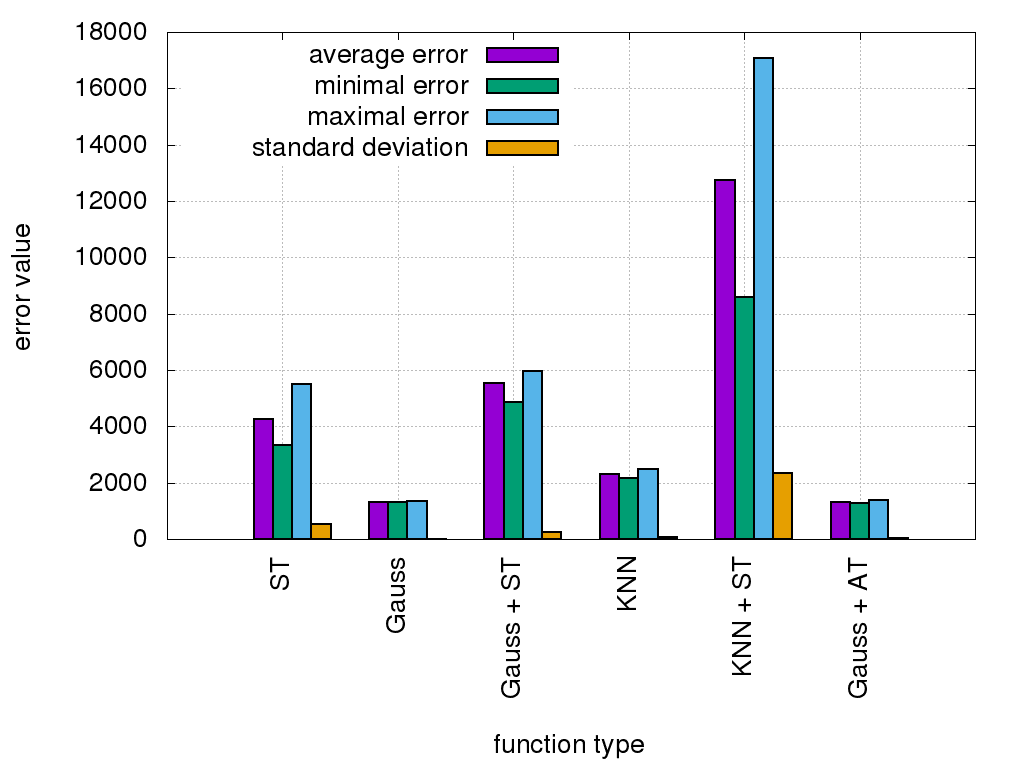
\includegraphics[scale=.36]{../../results_q_learning/map_3/trials_average_results.png}
\end{figure}

\end{frame}






\begin{frame}{\bf Praktický experiment - robot sledujúci čiaru}

\begin{figure}[!htb]
\centering
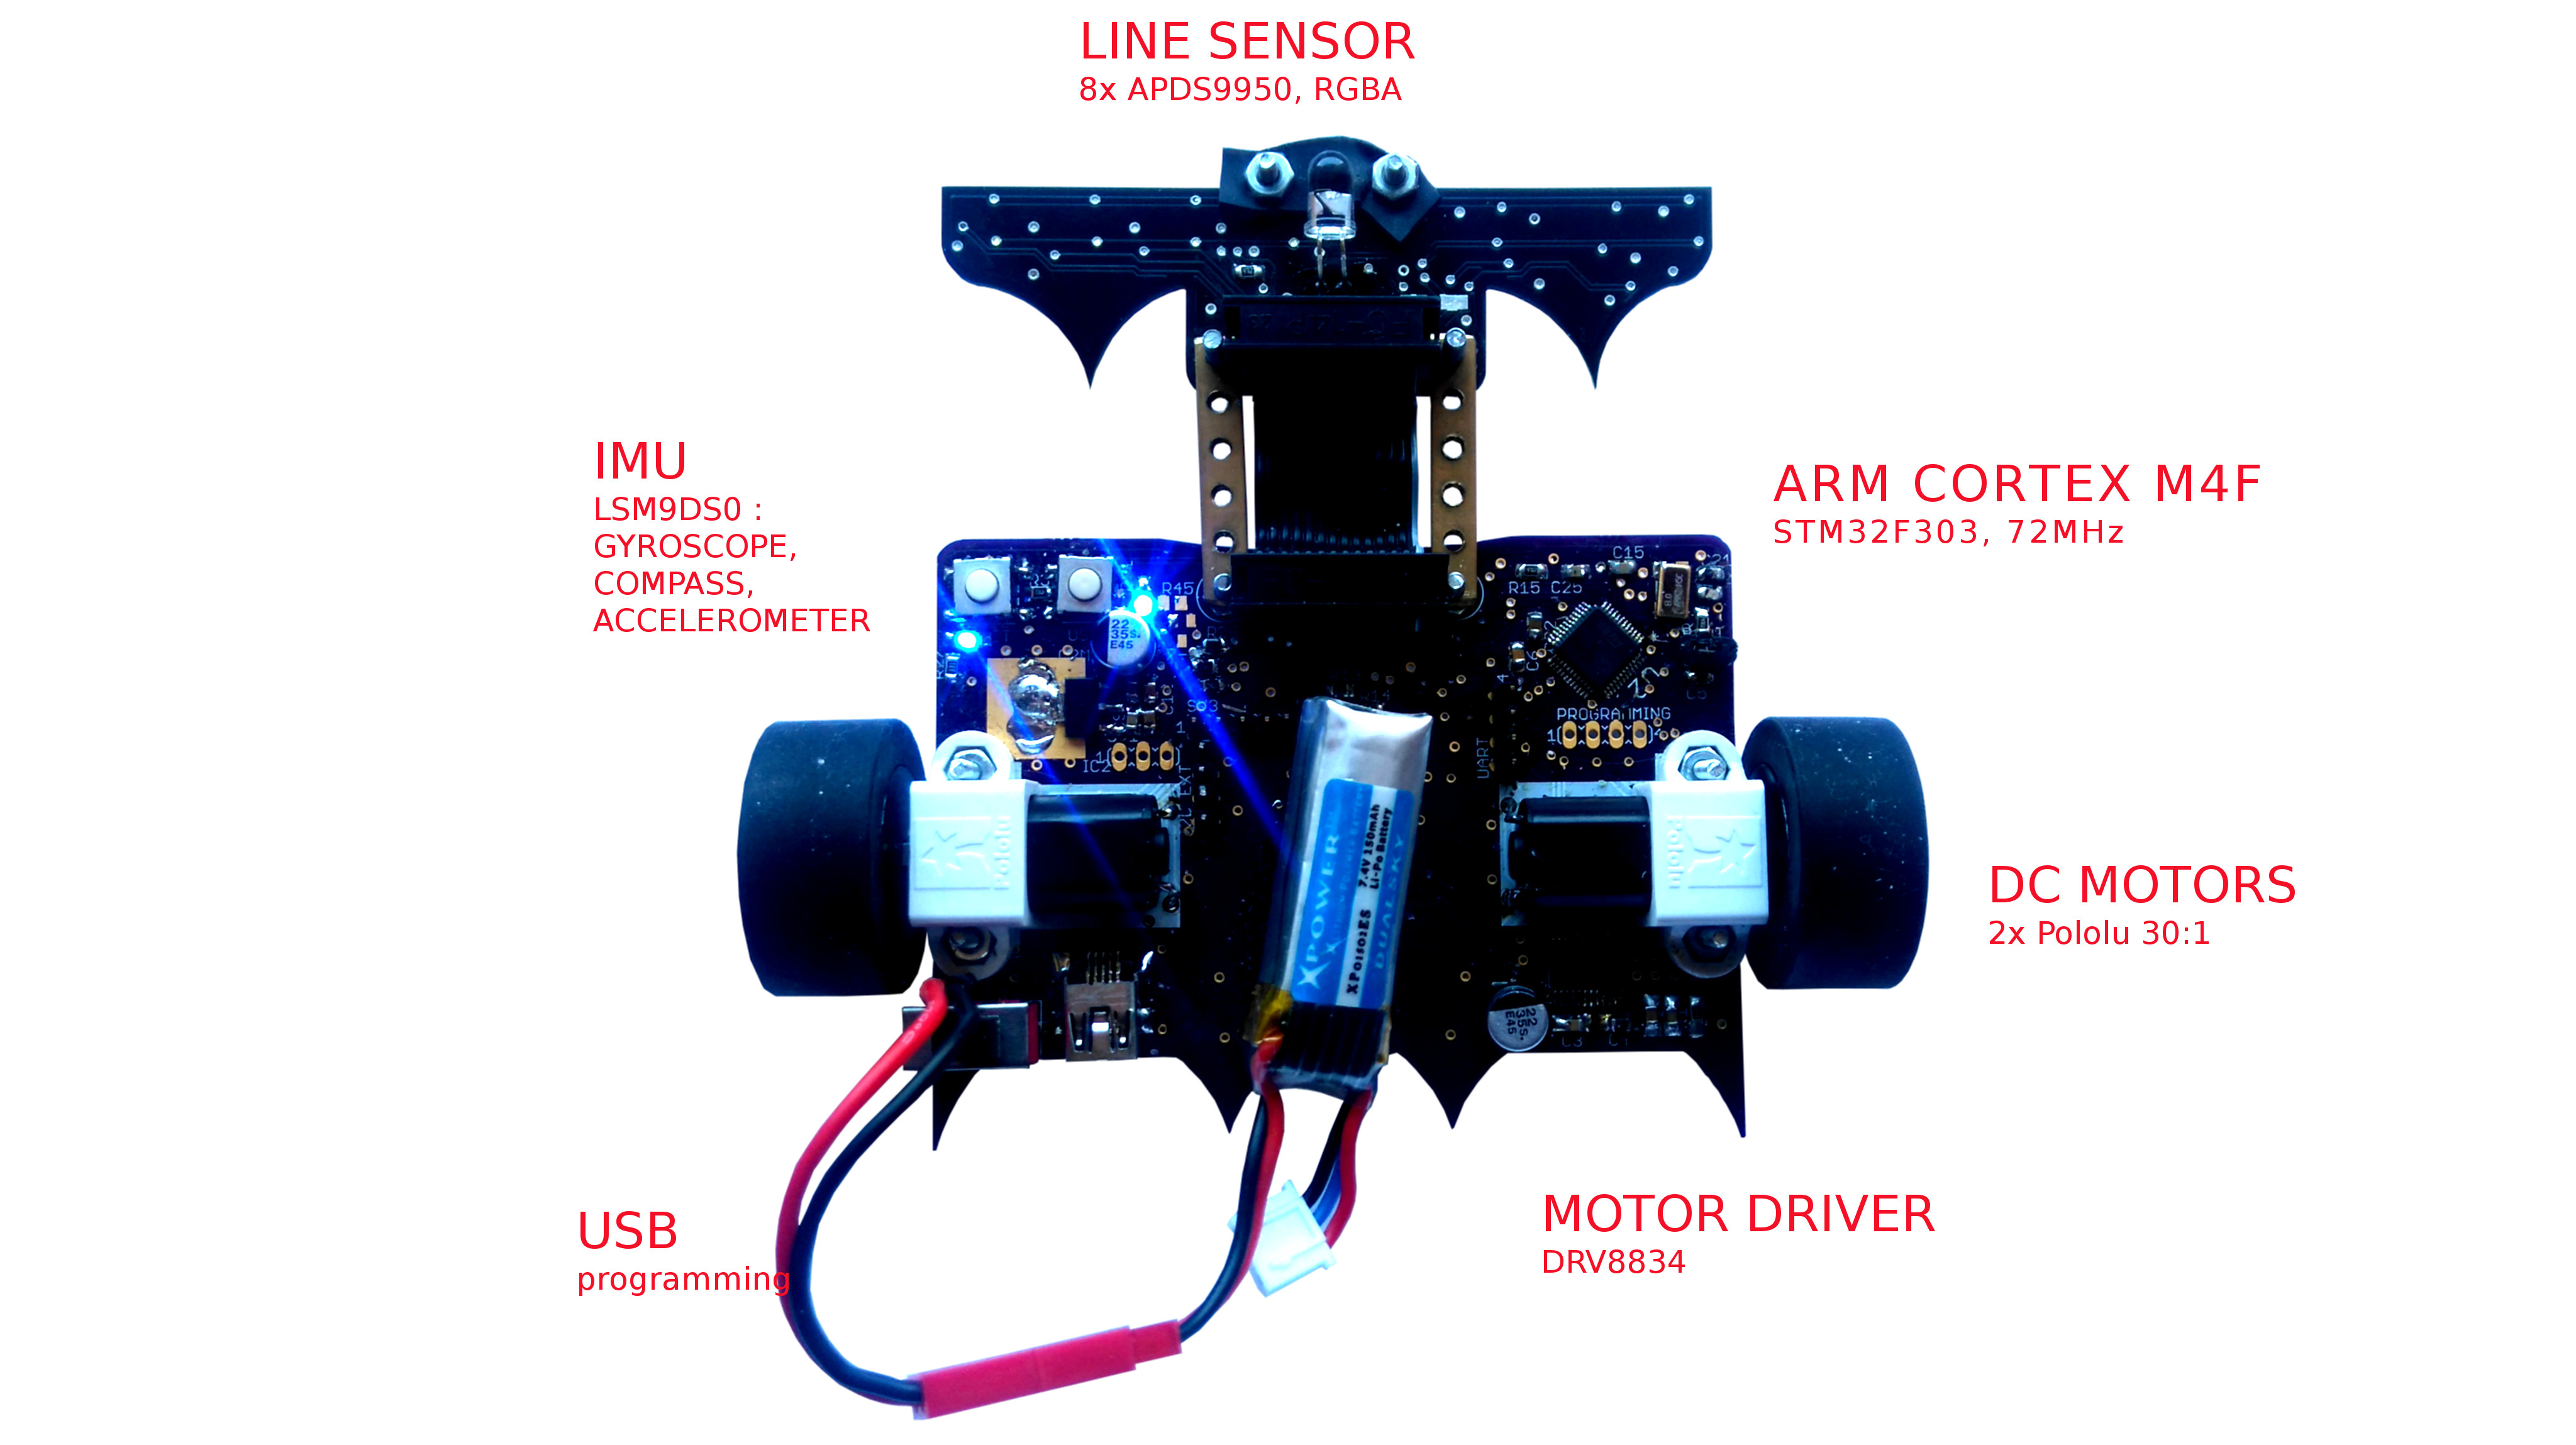
\includegraphics[scale=.09]{../pictures/robot_hardware_white.jpg}
%\caption{robot motoko foto}
%\label{img:peak_and_hill_path}
\end{figure}

\end{frame}

\begin{frame}{\bf Praktický experiment - robot sledujúci čiaru}

\begin{enumerate}
 \item senzorová úroveň : \textcolor{blue}{interpolácia z 8 RGB senzorov + filtrácia}
 \item vrchná úroveň : \textcolor{ForestGreen}{stanovenie žiadanej hodnoty pomocou Q learning}
 \item spodná úroveň : \textcolor{red}{riadenie dvojicou PD + PI}
\end{enumerate}

\begin{figure}[!htb]
\centering
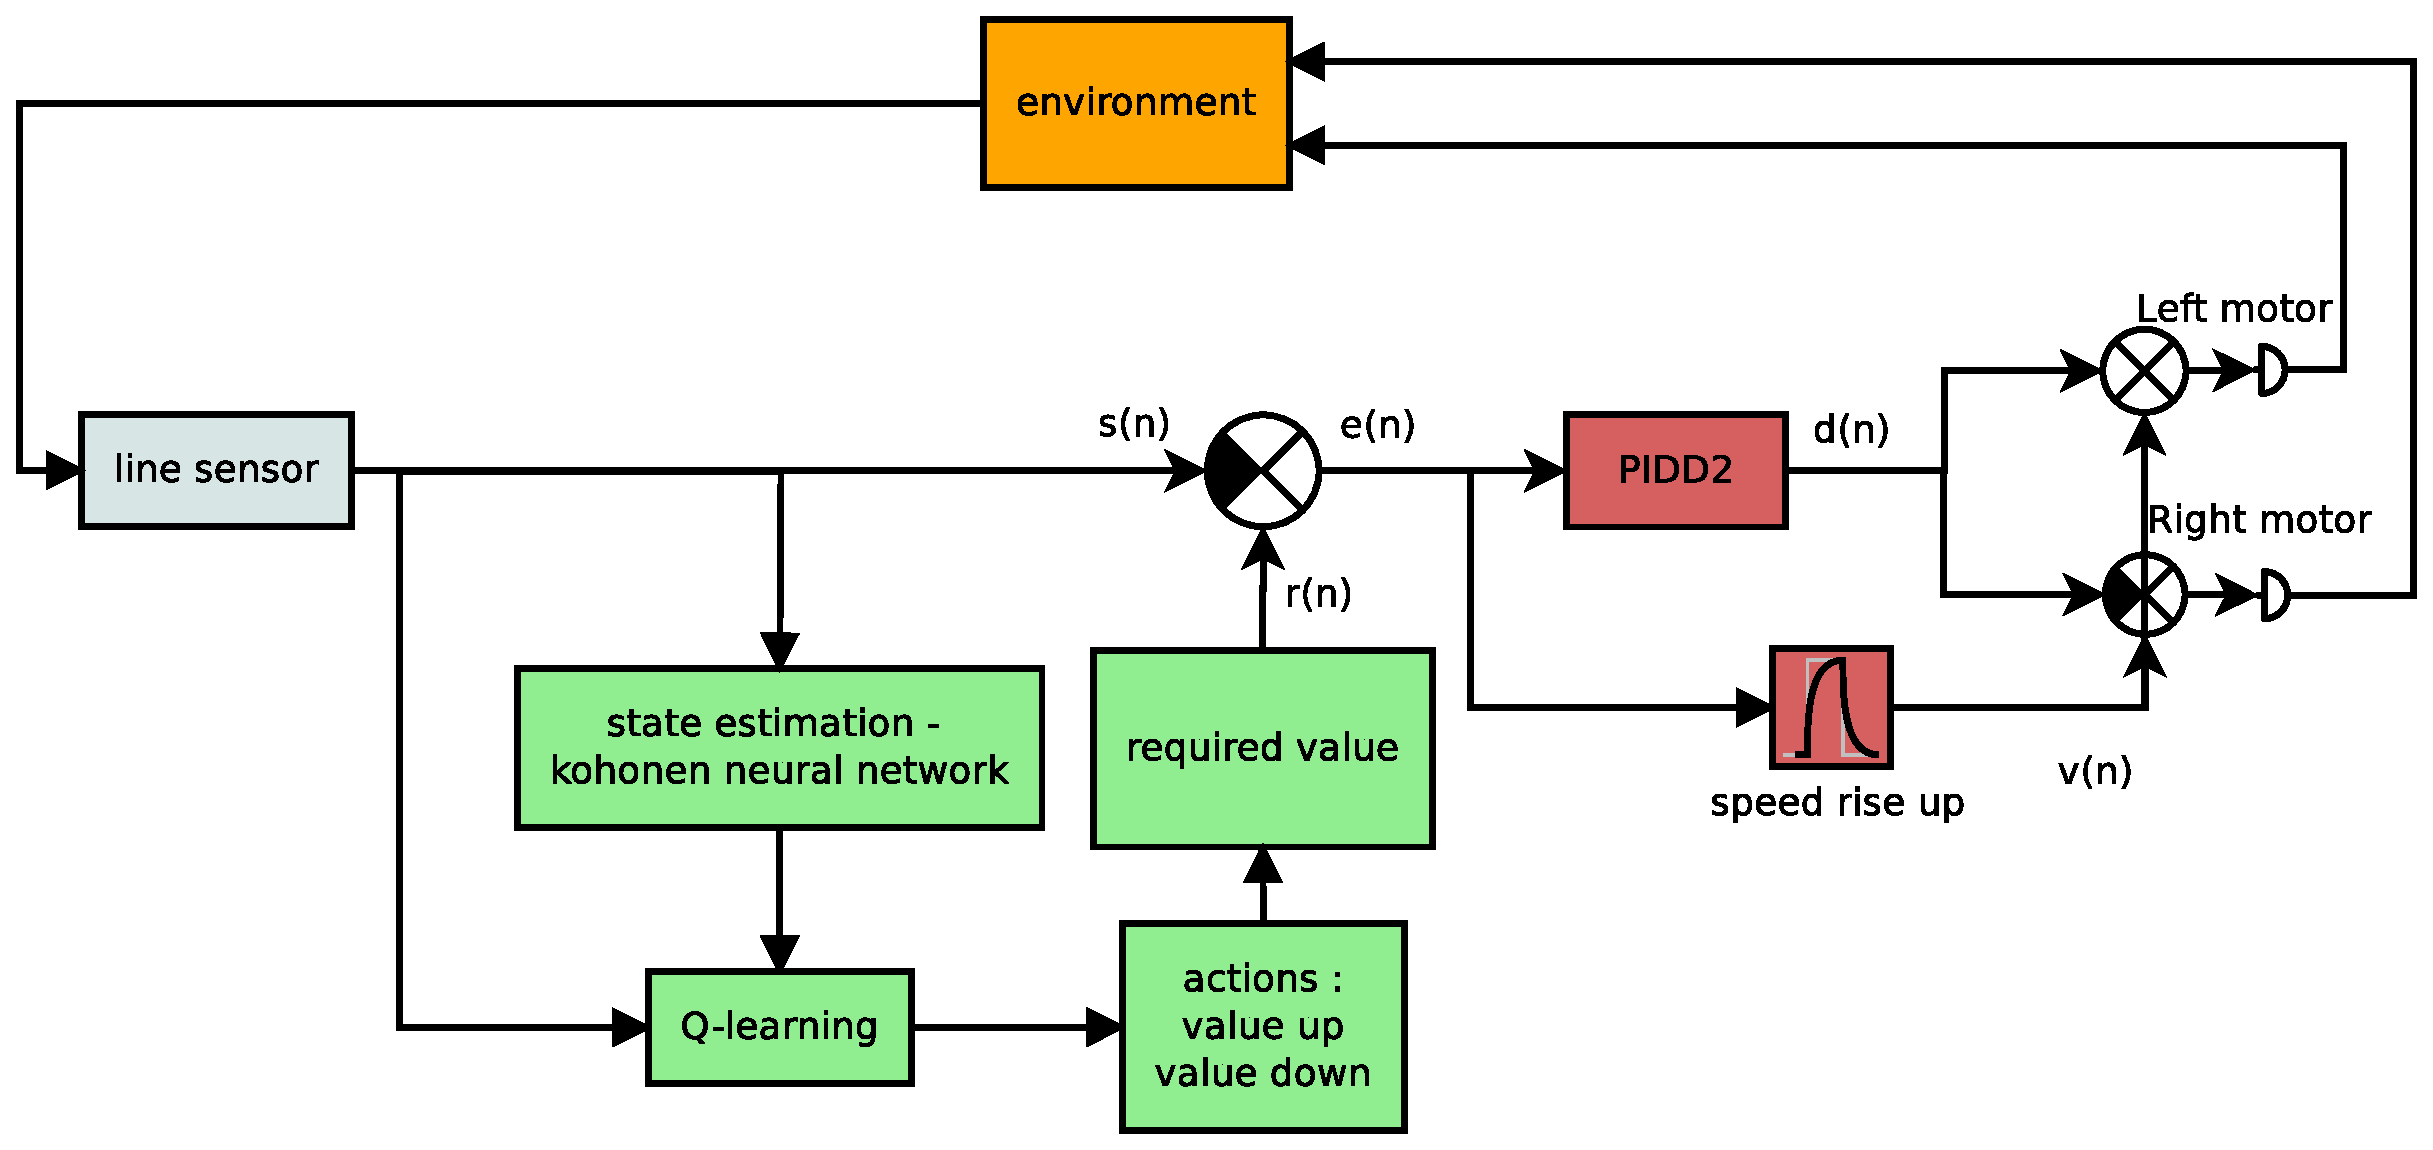
\includegraphics[scale=.2]{../diagrams/motoko_robot_block.eps}
\caption{Bloková schéma riadiaceho bloku robota}
\label{img:motoko_robot_block}
\end{figure}


\end{frame}

\begin{frame}{\bf Ďalšie smerovanie - sparse distributed memory (SDM)}
\begin{enumerate}
 \item sparse distributed memory {(\footnotesize Pentti Kenerva 1988)}
 \item  hierarchical temporal memory {(\footnotesize Jeff Hawkins 2012 )}
 \item adaptive sparse distributed memory {(\footnotesize Michal Chovanec 2016, v tlači)}
\end{enumerate}
\bigskip
aproximácia
$D(n) = f( A(n) )$
\begin{figure}[!htb]
\centering
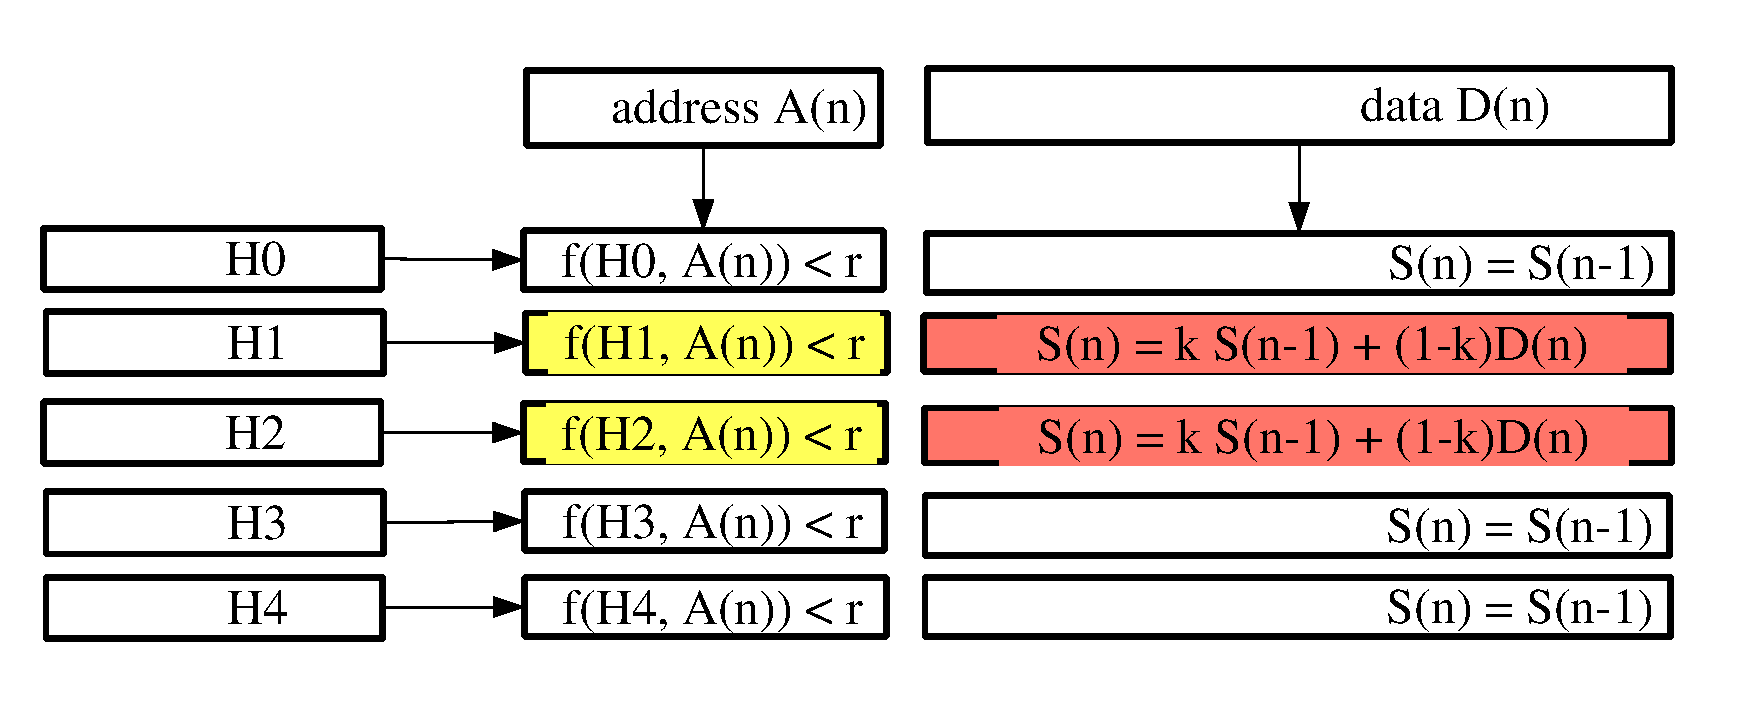
\includegraphics[scale=.4]{../pictures/sdm.pdf}
\label{img:motoko_robot_block}
\end{figure}
\end{frame}


\begin{frame}{\bf Adaptive sparse distributed memory}

Pokrytie priestoru s hard locations (3D rez 50D priestoru) pre dáta
s nerovnomerným rozdelením pravdepodobnosti

\begin{minipage}{.5\textwidth}

\begin{figure}[!htb]
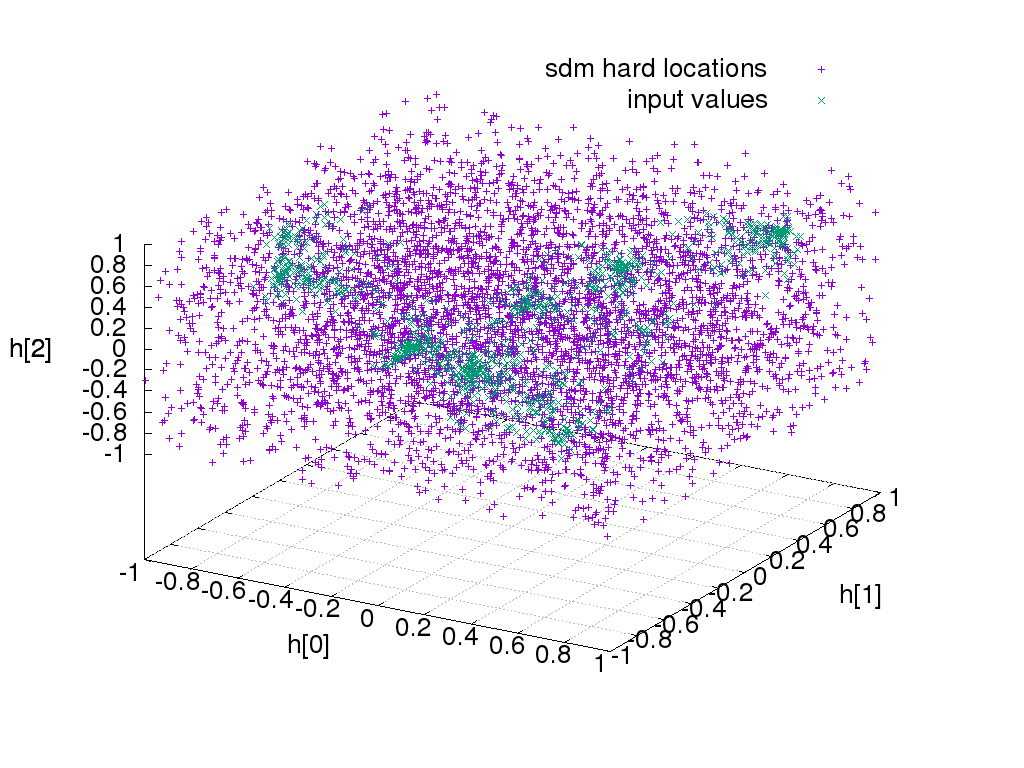
\includegraphics[scale=.25]{../pictures/sdm_hard_locations_all_original.png}
\caption{Slabé pokrytie}
\label{img:oroginal_sdm}
\end{figure}


\end{minipage}%
\begin{minipage}{.5\textwidth}

\begin{figure}[!htb]
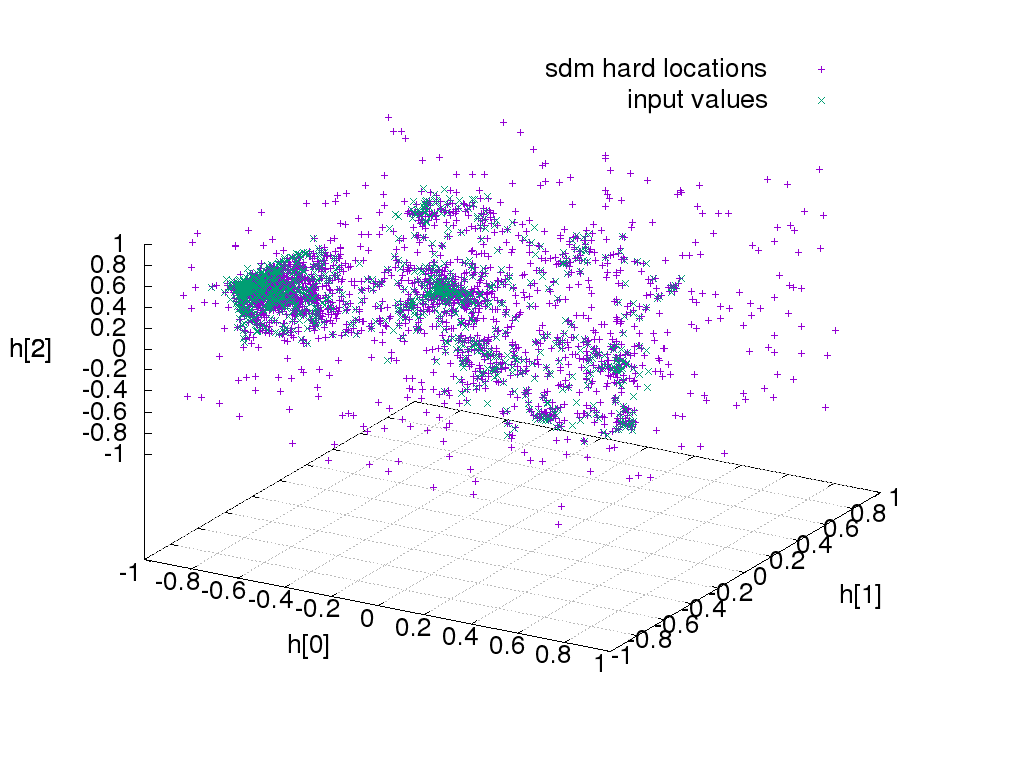
\includegraphics[scale=.25]{../pictures/sdm_hard_locations_all_new.png}
\caption{Vylepšené pokrytie}
\label{img:adaptive_sdm}
\end{figure}


\end{minipage}

\end{frame}




\begin{frame}{\bf Experimentálne výsledky}

- aproximácia funkcie, predikcia časových radov, MNIST - rukou písané číslice

\begin{figure}[!htb]
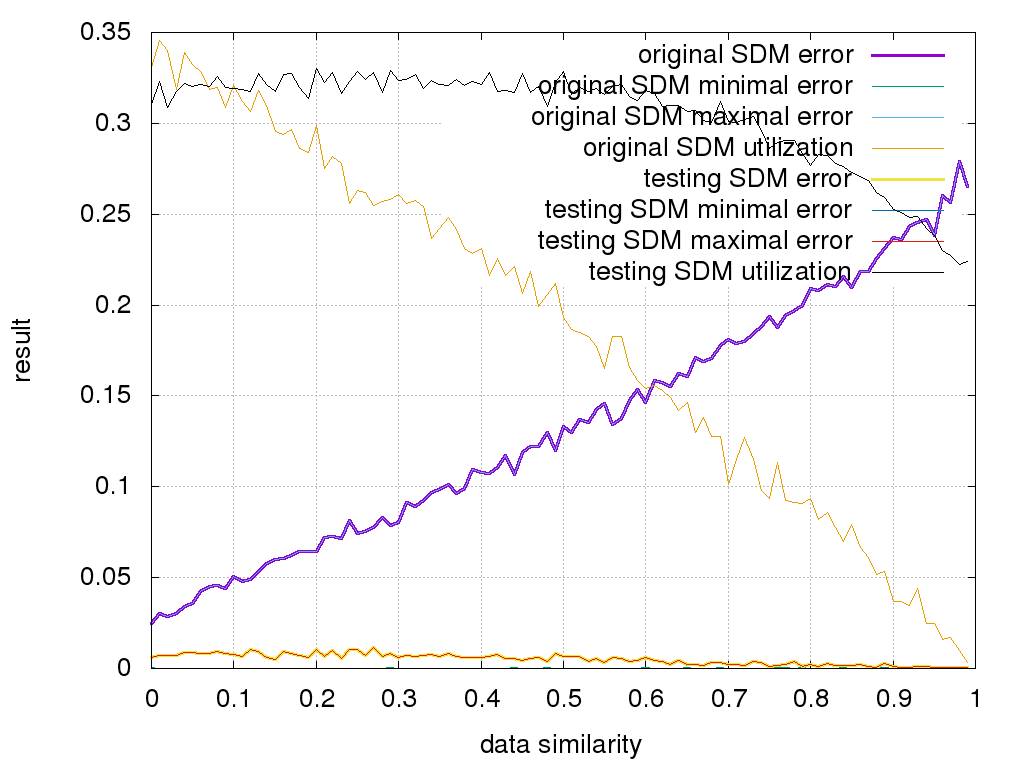
\includegraphics[scale=.35]{../pictures/aproximation_result_all.png}
\label{img:oroginal_sdm}
\end{figure}

\end{frame}


\begin{frame}{\bf Publikácie}
  	\tiny
\begin{enumerate}
  \item Intelligent traffic-safety mirror [Inteligentné dopravné zabezpečovacie zrkadlo] / M. Hodoň, M. Chovanec, M. Hyben.
  \item Intelligent traffic-safety mirror by using wireless sensor network [Inteligentné dopravno-bezpečnostné zrkadlo s použitím bezdrôtovej siete] / Peter Danišovič, Michal Hodoň, Michal Chovanec.
  \item Tiny low-power WSN node for the vehicle detection [Jednoduchý energeticky-efektívny nód bezdôtovej senzorovej siete určený na detekciu automobilov] / Michal Chovanec, Michal Hodon and Lukas Cechovic.
  \item Maximizing performance of low-power WSN node on the basis of event-driven-programming approach : Minimization of operational energy costs of WSN node control unit / Michal Hodoň ... [et al.].
  \item \textcolor{red}{Real-time schedule for mobile robotics and WSN aplications / Michal Chovanec, Peter Šarafín.}
  \item Universal synchronization algorithm for wireless sensor networks - FUSA algorithm / Michal Chovanec ... [et al.].
  \item \textcolor{red}{Investigation of the gyro-sensor contribution to the straight movement of vehicle [Analýza vplyvu gyroskopického senzora pri priamom pohybe vozidla] / Michal Hodoň, Michal Chovanec.}
  \item \textcolor{red}{Udalosťami riadené programovanie v OS Suzuha = Event driven programming in Suzuha OS / Michal Chovanec.}
  \item \textcolor{red}{Required value classification using Kohonen neural network = Klasifikácia žiadanej hodnoty Kohonenovou neurónovou sieťou / Michal Chovanec.}
  \item Akcelerometrické meranie výstrelu z luku = Accelerometrics measuring bow shot / Michal Chovanec a Jaroslav Múčka.
  \item Wireless sensor networks for intelligent transportation systems / Michal Hodoň, Juraj Miček, Michal Chovanec.
  \item \textcolor{red}{Signal mixing using neural network / Michal Chovanec.}
  \item \textcolor{red}{Adaptive sparse distributed memory as function approximator / Michal Chovanec, Peter Šarafín} - v tlači
  \item \textcolor{red}{Aeris – robots laboratory with dynamic environment / Michal Chovanec, Lukáš Čechovič and Lukáš Mandák} - v tlači
\end{enumerate}


\end{frame}


%-------------------------------------------------------------------------------------
\begin{frame}{\bf Ďakujem za pozornosť}

\centerline{michal.chovanec@yandex.ru}
\centerline{https://github.com/michalnand/q\_learning}

\begin{figure}[!htb]
\centering
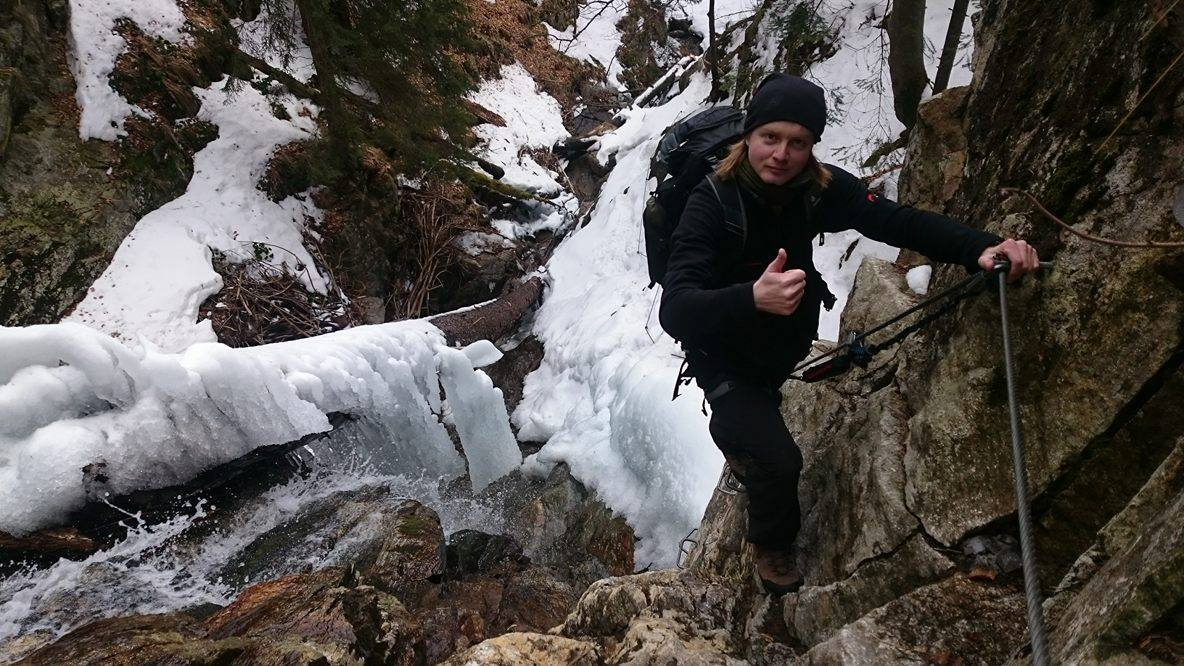
\includegraphics[scale=.25]{../pictures/me_ferrata.jpg}
%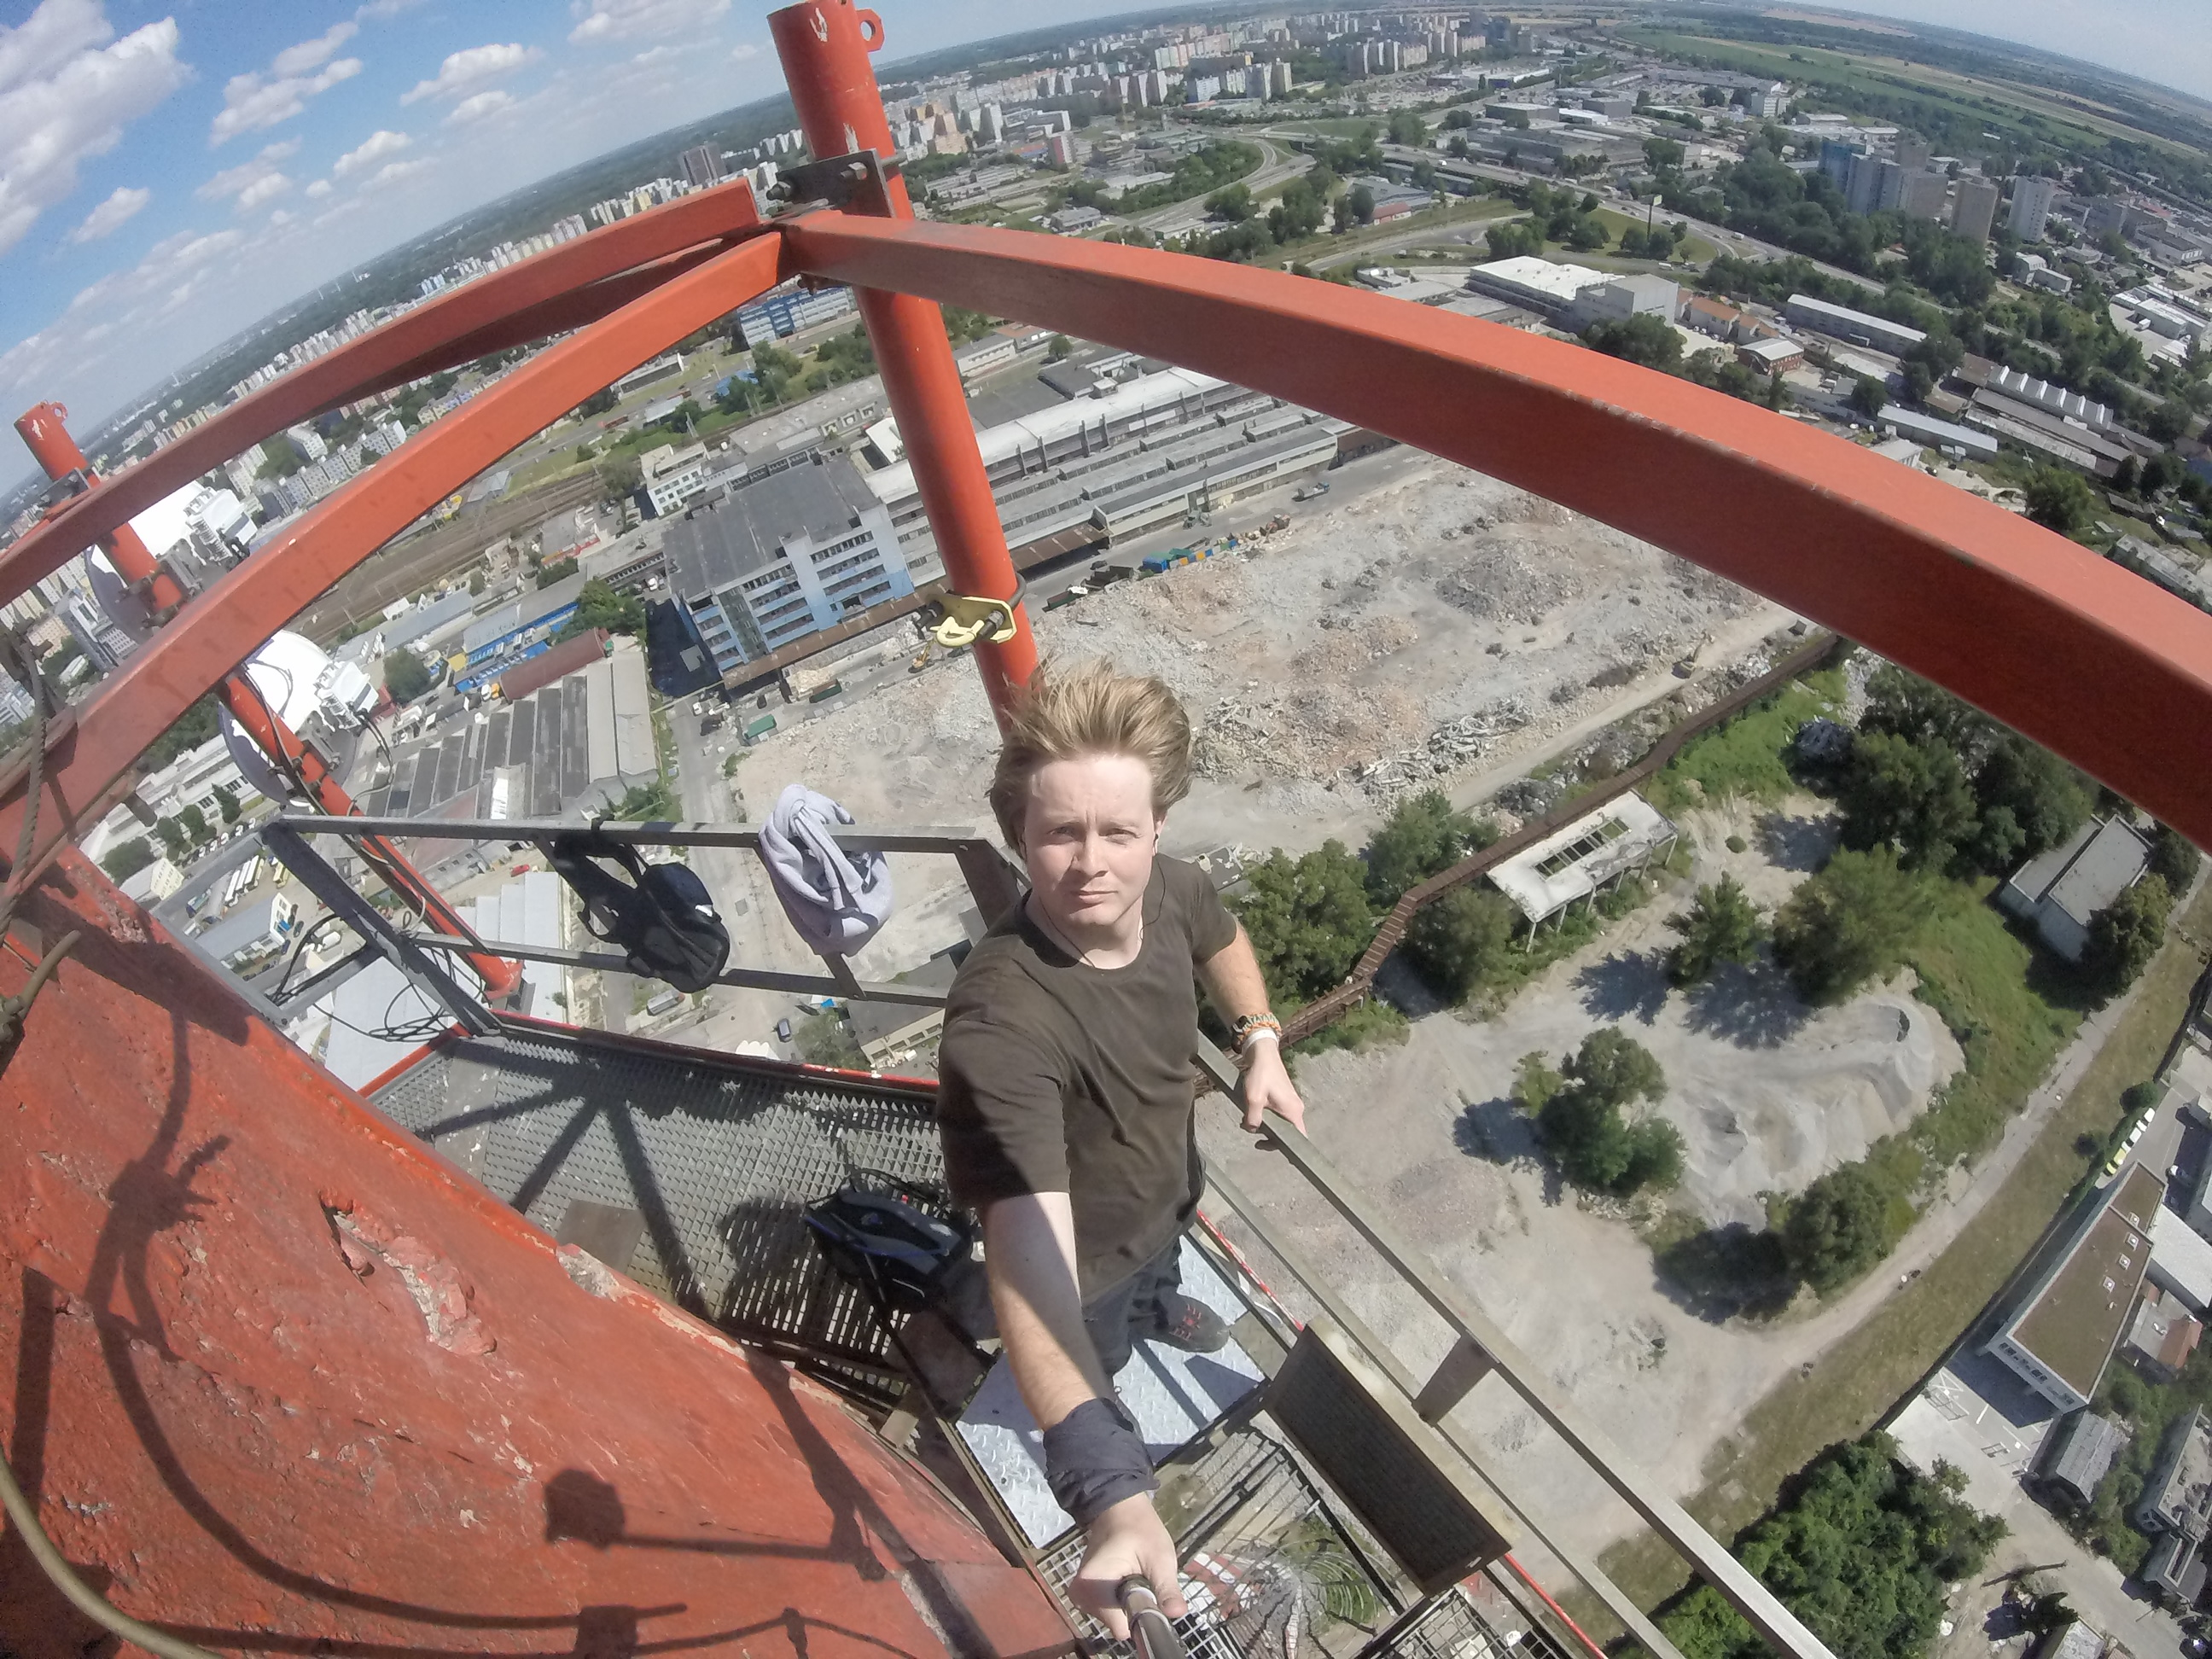
\includegraphics[scale=.1]{../pictures/me_chimney.jpg}
\end{figure}



\end{frame}

\end{document}
